  \documentclass[english,msc,numbers,hidelinks]{coppe}

\usepackage{amsmath,amssymb}
\usepackage{hyperref}
\usepackage{longtable}
\usepackage{booktabs}
\usepackage{float}
%\floatplacement{figure}{H}

% Change to Captions
\usepackage{caption}
\usepackage[font=footnotesize,labelfont={it}]{caption}

\providecommand{\tightlist}{%
  \setlength{\itemsep}{0pt}\setlength{\parskip}{0pt}}

\makelosymbols
\makeloabbreviations


% From {rticles}
\newlength{\csllabelwidth}
\setlength{\csllabelwidth}{3em}
\newlength{\cslhangindent}
\setlength{\cslhangindent}{1.5em}
% for Pandoc 2.8 to 2.10.1
\newenvironment{cslreferences}%
  {}%
  {\par}
% For Pandoc 2.11+
% As noted by @mirh [2] is needed instead of [3] for 2.12
\newenvironment{CSLReferences}[2] % #1 hanging-ident, #2 entry spacing
 {% don't indent paragraphs
  \setlength{\parindent}{0pt}
  % turn on hanging indent if param 1 is 1
  \ifodd #1 \everypar{\setlength{\hangindent}{\cslhangindent}}\ignorespaces\fi
  % set entry spacing
  \ifnum #2 > 0
  \setlength{\parskip}{#2\baselineskip}
  \fi
 }%
 {}
\usepackage{calc} % for calculating minipage widths
\newcommand{\CSLBlock}[1]{#1\hfill\break}
\newcommand{\CSLLeftMargin}[1]{\parbox[t]{\csllabelwidth}{#1}}
\newcommand{\CSLRightInline}[1]{\parbox[t]{\linewidth - \csllabelwidth}{#1}}
\newcommand{\CSLIndent}[1]{\hspace{\cslhangindent}#1}
\begin{document}

  \title{Titulo de Tese}
  \foreigntitle{Thesis' Title}
    \author{Jefferson T.}{Silvério}
      \advisor{Prof.}{Gisele A.}{Oda}{D.Sc.}
    \advisor{Prof.}{Verónica}{Valentinuzzi}{Ph.D}
    \advisor{Prof.}{Patricia}{Tachinardi}{Ph.D}
  

    \examiner{Prof.}{Nome Completo do Primeiro Examinador}{D.Sc.}
    \examiner{Prof.}{Nome Completo do Segundo Examinador}{Ph.D}
    \examiner{Prof.}{Nome Completo do Terceiro Examinador}{Ph.D}
    \department{IB}
  \date{10}{2021}
    \keyword{Primeira palavra-chave}
    \keyword{biologging}
    
  % Adiciona Pagina de Titulo
  \maketitle

  % Adiciona Pagina de Rosto com 
  \frontmatter
  
  %Adiciona dedicatorias
  \dedication{A alguém cujo valor é digno desta dedicatória.}
    \chapter*{Agradecimentos}
  Gostaria de agradecer a X
  
  % Adiciona Abstracts
  \begin{abstract}
  ABSTRACT
  \end{abstract}
  \pagebreak
  \begin{foreignabstract}
  ABSTRACT INGLES
  \end{foreignabstract}
  % Adiciona Sumário
  \tableofcontents
  
  % Adiciona Lista de Figuras
    \listoffigures
  
  % Adiciona Lista de Tabelas
    \listoftables
  
  % Adiciona Lista de Simbolos e Abreviacoes
  \printlosymbols
  \printloabbreviations

  % Adiciona Corpo da Tese
  \mainmatter
  \hypertarget{hidden-markov-models-reveals-annual-changes-in-the-daily-activity-levels-of-the-anillaco-tuco-tuco-ctenomys-sp.}{%
  \chapter{\texorpdfstring{Hidden Markov Models reveals annual changes in the daily activity levels of the Anillaco Tuco-tuco (\emph{Ctenomys sp.})}{Hidden Markov Models reveals annual changes in the daily activity levels of the Anillaco Tuco-tuco (Ctenomys sp.)}}\label{hidden-markov-models-reveals-annual-changes-in-the-daily-activity-levels-of-the-anillaco-tuco-tuco-ctenomys-sp.}}

  \hypertarget{introduction}{%
  \section{Introduction}\label{introduction}}
  \begin{itemize}
  \tightlist
  \item
    Contexto:
  \item
    Síntese do conhecimento:O que se sabe sobe o tema central?
  \item
    Como a questão investigada se encaixa nesse contexto teórico?
  \item
    Rever anotações
  \item
    objetivos: - tbm testar a necessidade de classificar para ritmicidade
  \end{itemize}
  \hypertarget{methods}{%
  \section{Methods}\label{methods}}

  \hypertarget{study-species}{%
  \subsection{Study Species}\label{study-species}}

  The studied \emph{Ctenomys} population lacks a formal phylogenetic and taxonomic classification but there are some lines of evidence suggesting that the study area is occupied by a single unidentified species (\protect\hyperlink{ref-amaya2016}{Amaya et al. 2016}). In other studies, the studied \emph{Ctenomys'} species has been referred informally as the Anillaco tuco-tuco (\protect\hyperlink{ref-amaya2016}{Amaya et al. 2016}) and as \emph{Ctenomys} aff. \emph{knightii} (\protect\hyperlink{ref-tomotani2012}{Tomotani et al. 2012}) or \emph{Ctenomys} cf.~\emph{knightii} (\protect\hyperlink{ref-valentinuzzi2009}{Valentinuzzi et al. 2009}).

  \hypertarget{study-site}{%
  \subsection{Study Site}\label{study-site}}

  Field work was conducted at a site located approximately 5km away from the village of Anillaco, in the province of La Rioja, Northwest Argentina. The study site (-66.95°, -028.80, 1325m; Figure \ref{fig:methods-map}) is a relatively undisturbed natural area, with little human disturbance and no artificial light source. The area is surrounded by the Sierra de Velasco mountain range, located within the Monte Desert biome. The Monte Desert is characterized as an open shrubland dominated by Zygophyllaceae (\emph{Larrea cuneifolia} Cav., \emph{Tricomaria usillo}), Fabaceae (\emph{Prosopis torquata}, \emph{Senna aphylla}) and Cactaceae (\emph{Trichocereus} spp, \emph{Tephrocactus} spp) (\protect\hyperlink{ref-abraham2009}{Abraham et al. 2009}; \protect\hyperlink{ref-fracchia2011}{Fracchia et al. 2011}; \protect\hyperlink{ref-aranda-rickert2011a}{Aranda-Rickert and Fracchia 2011}). At the study site a non-extensive survey of the plant community divided in three transects showed a dominance of the families Zygophyllaceae (\emph{Larrea cuneifolia}, \emph{Tricomaria usillo}), Poaceae (\emph{Microchloa indica}, \emph{Aristida mendocina}) and Fabaceae (\emph{Zuccagnia punctata}) (Figure \ref{fig:appendix-plants}). The climate is arid with marked daily and seasonal cycles in temperature and rainfall (Figure \ref{fig:appendix-weather}). The mean annual temperature is 16.6°C (\protect\hyperlink{ref-fracchia2011}{Fracchia et al. 2011}), with clear differences in the daily range and between summer and winter months (\protect\hyperlink{ref-abraham2009}{Abraham et al. 2009}). The mean annual rainfall ranges from 145 to 380mm concentrated almost exclusively in the summer months (\protect\hyperlink{ref-fracchia2011}{Fracchia et al. 2011}).
  \begin{figure}

  {\centering 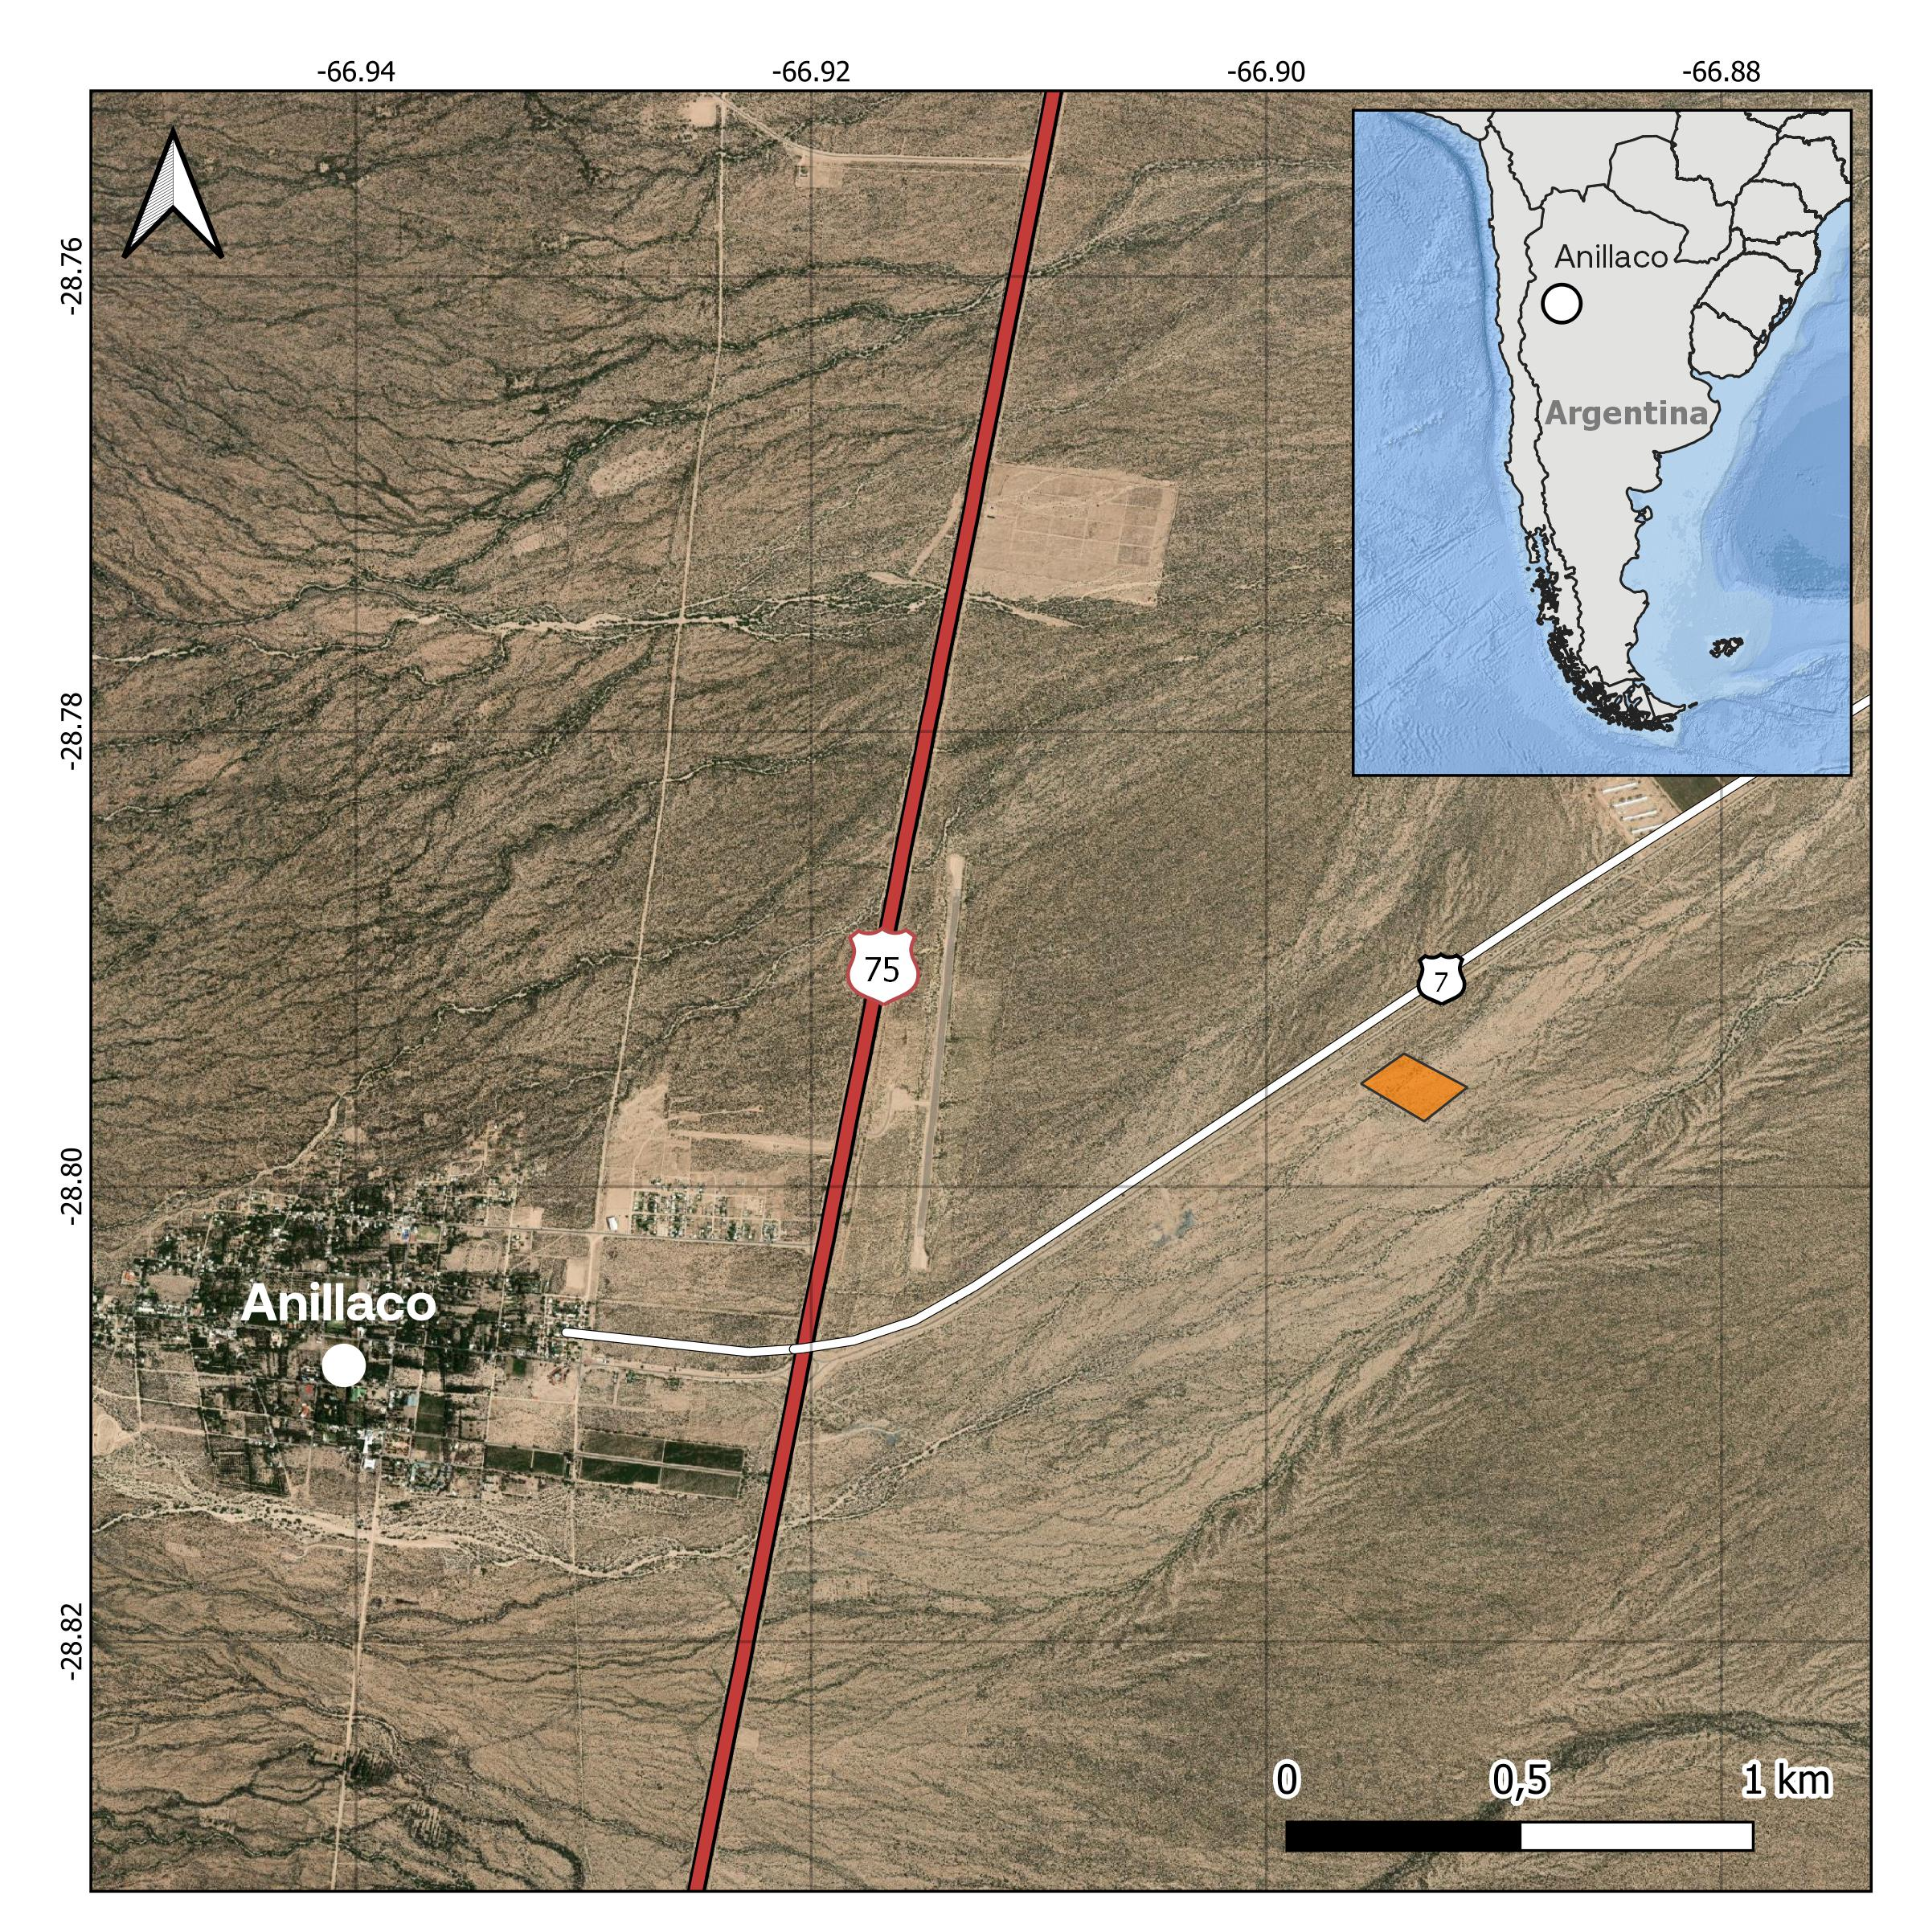
\includegraphics[width=1\linewidth]{../04_figures/map/tuco_map} 

  }

  \caption{Study site location (orange icon) at the Monte Desert, approximately 5km away from the village of Anillaco, northwest of Argentina}\label{fig:methods-map}
  \end{figure}
  \hypertarget{animal-capture-and-handling}{%
  \subsection{Animal Capture and Handling}\label{animal-capture-and-handling}}

  A total of 47 tuco-tucos were captured between March 2019 and March 2020. Out of these, 30 were part of the present study. Trapping was conducted in four different campaigns to the study site. Three campaigns were done in 2019 during March-April (Autumn), July (Winter) and October (Spring). A fourth campaign was done in February 2020 (Summer). A fifth campaign was planned to occur in May 2020 but had to be canceled due to the COVID-19 outbreak. Tuco-tucos were captured using a custom-made PVC pipe trap (35cm length, 10cm diameter) with a spring-loaded aluminum door at one end and a cul-de-sac at the other. Before setting the traps, the study site was scouted for active tuco-tuco's burrows. Active burrows could be identified by the presence of freshly excavated soil mounds at the burrow's entrance. Once found, burrows were excavated to open the access to the underground tunnels and a trap was placed horizontally at the burrow's entrance following the tunnel's orientation. Traps were placed at all active burrows found at the study site, limited to a max of 20 traps available. Traps were set in the field during the morning and checked every 2 hours, when they were reset if they had been plugged with soil or if they had been activated without any tuco-tuco capture. Traps were checked for a last time at dusk and then taken out if no animal had been caught.

  After capture, adult tuco-tucos (\textgreater120g) were lightly anesthetized in order to be carefully examined and receive a biologging collar. We used a clear plastic anesthesia chamber (318.5cm³) with a clip-on lid and a cotton ball affixed inside of the chamber, out of the animal's reach. The cotton ball received approximately 0.5 mL of isoflurane before transferring the animal from the trap to the chamber. While in the chamber animals were observed for breathing, blinking and loss of righting reflex. Once the tuco-tucos could not right themselves they were removed from the chamber. Anesthetized animals were weighted (CSseries, OHAUS, ± 1 g precision), sexed, assessed for reproductive status, marked with a subcutaneous identification PITTag (Passive Integrative Transponder. Allflex, Brasil) and fitted with a collar bearing biologgers (See Activity Sensors).

  Animals were released in the same burrow they were originally captured. They were left in the field for 5-18 days before being recaptured for collar recovery. The telemetry transmitter was used to maximize animal localization, thus avoiding the loss of the other devices. All animal captures, procedures and animal handling were authorized by the local authorities at \emph{Dirección General de Ambiente y Desarrollo Sustentable -- Secretaría de Ambiente del Ministerio de Producción y Desarollo Local} -- La Rioja, Argentina (\#00501-17). All procedures were also approved by the Ethics Committee at the \emph{Instituto de Biociências} (\#308-2018) and \emph{Faculdade de Medicina Veterinária} (\#2045300519) of the \emph{Universidade de São Paulo}.

  \hypertarget{biologgers}{%
  \subsection{Biologgers}\label{biologgers}}

  Accelerometers (Axy-4, TechnoSmart, Italy) and lightloggers (W65, Migrate Technology, UK) were used to record general motor activity and light exposure, respectively. These biologgers were attached to a collar made of a cable tie inserted through silicon tubing (\protect\hyperlink{ref-jannetti2019}{Jannetti et al. 2019}; \protect\hyperlink{ref-williams2014}{Williams et al. 2014}, Figure \ref{fig:methods-collar}). A telemetry transmitter (SOM-2011. Wildlife Materials, USA) was also attached to the collar to assist in animal location during recapture and minimize sensor's loss. The complete collar setup (accelerometer, lightlogger and telemetry) weighted approximately a total of 6g. Collars without the lightlogger weighted 5.3g. All accelerometers recorded tri-axial acceleration at a 10Hz sampling frequency and 4G sensitivity. Lightloggers were set to sample illuminance every minute but only recorded the maximum sampled value each 5 minutes. The lighlogger possible recording range was 1-19000 lux.
  \begin{figure}

  {\centering 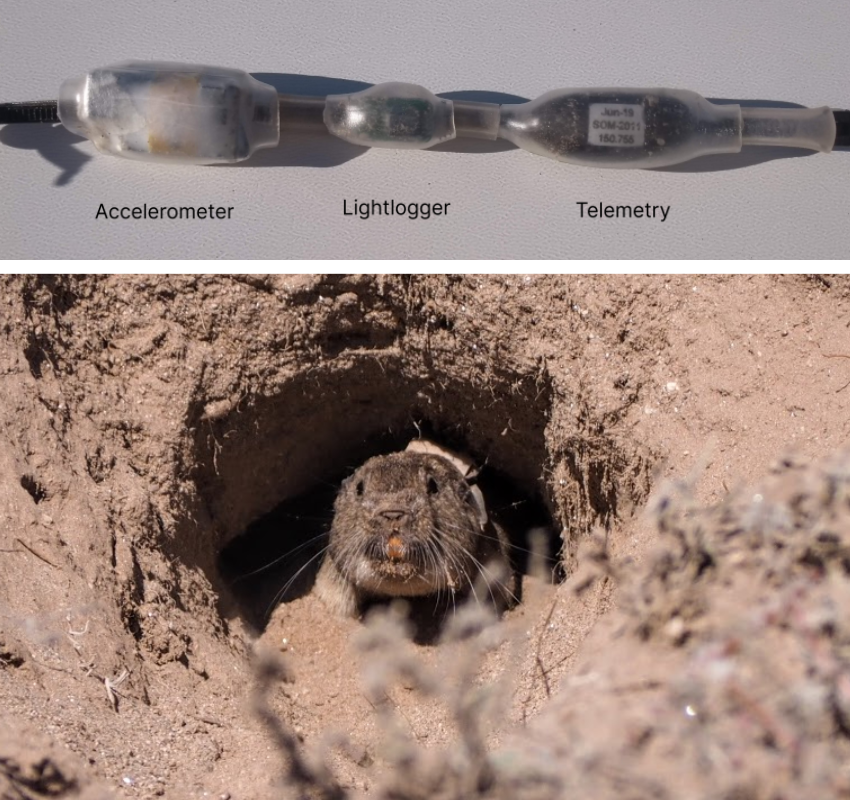
\includegraphics[width=1\linewidth]{../04_figures/collar/collar_tuco} 

  }

  \caption{Collar setup and example of field deployment. Upper photo shows the complete collar setup with accelerometer, lightlogger and the telemetry transmitter. Bottom photo shows a tuco-tuco wearing a collar. In the bottom photo it is possible to see the acceleromer and the lightlogger attached to the collar.}\label{fig:methods-collar}
  \end{figure}
  \hypertarget{data-processing-general-activity-calculation}{%
  \subsection{Data Processing \& General Activity Calculation}\label{data-processing-general-activity-calculation}}

  Data were recorded on board of the sensors and later downloaded and converted to raw text files using the software provided by the device's manufacturers. Acceleration data was used to measure gross motor activity. Tri-axial acceleration data was first reduced to one dimension using the Vectorial Dynamic Body Acceleration (VeDBA, \protect\hyperlink{ref-qasem2012}{Qasem et al. 2012}). VeDBA is commonly used as a proxy for the animal's activity level and energy expenditure (\protect\hyperlink{ref-wilson2008}{Wilson et al. 2008}; \protect\hyperlink{ref-williams2016}{Williams et al. 2016}). VeDBA was calculated by: (i) Estimating the effect of the gravitational force over the accelerometer, also known as static acceleration. The static acceleration can be estimated by applying a moving average over the raw acceleration data. There is not a consensus over the number of points to calculate the moving average with, which can be dependent on the study species and device's recording frequency. In this study we used a 4-second moving average after following the methodology proposed by (\protect\hyperlink{ref-ref}{\textbf{ref?}}). (ii) Calculating the acceleration correspondent to the animal's movement, also known as Dynamic Body Acceleration (DBA). The DBA was calculated by subtracting the static acceleration from the raw data. (iii) Lastly, we calculate the VeDBA by the vectorial sum of the DBA over the device's axes.

  \[ VeDBA = \sqrt{Xd^2 + Yd^2 + Zd^2} \]

  Once VeDBA was calculated, the 1Hz acceleration data was downsampled by taking the median over a 1-minute non-overlapping sliding window. All VeDBA datapoints were classified as occurring during the daytime or nighttime based on the daylength of the recording dates. Daylength was calculated using the \emph{maptools} package in R (\protect\hyperlink{ref-bivand2020}{Bivand and Lewin-Koh 2020}), which uses the National Oceanic and Atmospheric Administration (NOAA) equations for estimating twilight times. We used civil twilight times, defined as the times in which the center of the sun is 6° below the horizon, as thresholds to calculate daylength and classify datapoints as occurring during the day or nighttime. Daylength change along the year at the study site can be seen in the Appendix (Figure \ref{fig:appendix-daylenght}).

  Light exposure was used to analyse the time tuco-tucos spend on the surface and to further classify VeDBA data points as above or below ground. The threshold for considering a data point as being aboveground was 2 lux, consistent with what has been done in \protect\hyperlink{ref-jannetti2019}{Jannetti et al.} (\protect\hyperlink{ref-jannetti2019}{2019}). Accelerometer and lightlogger data were merged accordingly to the date and times of recordings using purposely written R scripts (\protect\hyperlink{ref-rcoreteam2020}{R Core Team 2020}). Time of recordings between both devices were not synchronized to the minute. Consequently, we had to round lightlogger recording times to the nearest 5 minutes to merge both data streams.

  In order to exclude any effects that capture and recapture can have in the animal's activity, we removed the first and last days of all dataset. We also excluded the data corresponding to the days we were attempting to recapture the animal in cases where the recapture attempts took longer than one day. Animals that had data excluded due to recapturing efforts were FEV05 (5 days), JUL16 (5 days) and JUL23 (2 days).

  \hypertarget{time-on-surface-general-activity-analysis}{%
  \subsection{Time on Surface \& General Activity Analysis}\label{time-on-surface-general-activity-analysis}}

  VeDBA data was first used to analyse the general activity levels of tuco-tucos. The temporal distribution of VeDBA was visualized

  \hypertarget{hidden-markov-models}{%
  \subsection{Hidden Markov Models}\label{hidden-markov-models}}

  We used Hidden Markov Models (HMMs) to further analyze and classify the 1-minute VeDBA data. HMMs are a type of time series model, therefore, they take into account the temporal dependency of the observations (\protect\hyperlink{ref-leosbarajas2017}{Leos-Barajas et al. 2017}). Consequently, HMMs are well suited to model accelerometer data given their intrinsic temporal dependency (\protect\hyperlink{ref-leosbarajas2017}{Leos-Barajas et al. 2017}; \protect\hyperlink{ref-patterson2019}{A. Patterson et al. 2019}). HMMs are composed of two time series: the observable \emph{state-dependent process} (\(X_t\)), VeDBA in our case, and an underlying, or hidden, \emph{state process} (\(S_t\)). The \emph{state process} is what drives the observations and what we are interested in estimating, which roughly corresponds to behavioral states (Figure \ref{fig:hmm-formulation}).

  The \emph{state process} follows the Markov Property and take temporal dependency into account (\protect\hyperlink{ref-zucchini2016}{Zucchini, Iain MacDonald, and Roland Langrock 2016}). The Markov property denotes that a state \(S_t\) depends only on the previous state \(S_{t-1}\) (\protect\hyperlink{ref-zucchini2016}{Zucchini, Iain MacDonald, and Roland Langrock 2016}). In the case of accelerometer and animal movement studies the states are representations of the animals' behavior and can take on finite number (\(N\)) of possible values. The number of states can be chosen \emph{a priori} or based on model selection (\protect\hyperlink{ref-pohle2017}{Pohle et al. 2017}). The changes in probabilities between states are also part of the of HMM formulation, summarized by a Transition Probability Matrix that gives the probability of transitioning from the current state to a possible future state.

  In the basic HMM formulation the observable \emph{state-dependent process} comes from a mixture of \(N\) distributions, one for each state. These distributions come from a common family (e.g.~Normal, Weibull or Gamma) and each one have their own set of parameter values. The active distribution is determined by the state the system is in at a given time \(t\). Therefore, the observations are a realization from one of these distributions. The distribution parameters, state transition probabilities and other model parameters can be estimated by numerical maximization of the Likelihood (\protect\hyperlink{ref-zucchini2016}{Zucchini, Iain MacDonald, and Roland Langrock 2016}). With the model parameters in hand, the most probable state sequence can be found by the Viterbi algorithm (\protect\hyperlink{ref-mcclintock2020}{Brett T. McClintock et al. 2020}; \protect\hyperlink{ref-zucchini2016}{Zucchini, Iain MacDonald, and Roland Langrock 2016}).
  \begin{figure}

  {\centering 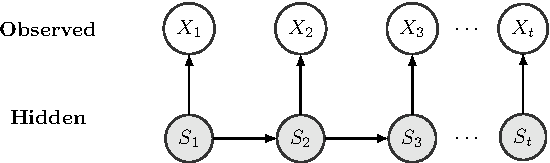
\includegraphics{tese_jefferson_files/figure-latex/hmm-formulation-1} 

  }

  \caption{Basic dependence structure for a Hidden Markov Model}\label{fig:hmm-formulation}
  \end{figure}
  \hypertarget{model-formulation-and-state-classification}{%
  \subsection{Model Formulation and State Classification}\label{model-formulation-and-state-classification}}

  In our models we have chosen VeDBA as our activity metric. We determined \emph{a priori} a possible number of three different states (\(N=3\)). This decision was made based on our research question, in the VeDBA distributions (REF Figure \ref{fig:appendix-eda}) and in the biological interpretability of the states. It is important to note, however, that the states do not correspond directly to specific behaviors (e.g.~feeding, foraging or digging) but can be assumed to roughly correspond to behavioral states (e.g.~activity levels) that can encompass a range of different behaviors (\protect\hyperlink{ref-leosbarajas2017}{Leos-Barajas et al. 2017}; \protect\hyperlink{ref-papastamatiou2018}{Papastamatiou et al. 2018}). We labelled the states as roughly corresponding to ``Rest,'' ``Medium Intensity Activity'' and ``High Intensity Activity.''

  HMMs can be fitted individually (e.g. \protect\hyperlink{ref-vandekerk2015}{van de Kerk et al. 2015}) or to a pool of animals (\protect\hyperlink{ref-langrock2012}{Langrock et al. 2012}). The models can also include covariate effects that modify either the \emph{state-dependent} distribution parameters or the transition probabilities (\protect\hyperlink{ref-patterson2009}{T. A. Patterson et al. 2009}; \protect\hyperlink{ref-langrock2012}{Langrock et al. 2012}). We fitted a 3-state HMM to the 1-minute VeDBA data using a `complete pooling' approach. This means that the \emph{state-dependent} distribution parameters are common to all animals. Therefore, we assume that individuals are independent and behaviors are the same to all individuals and across the year. However, given that the season/month of the year seems to be an important feature influencing the VeDBA distribution (Figure \ref{fig:appendix-eda}) we included season as a covariate in the \emph{state process}. Hence, nãwe let the probability of changing from one state to another vary in relation to the season/month of the year. We also fitted an empty model, with no covariate effects, and used Akaike's Information Criteria (AIC) to select the model with best fit to the data (\protect\hyperlink{ref-burnham2002}{Burnham, Anderson, and Burnham 2002}).

  Models were fitted using the momentuHMM package in R (\protect\hyperlink{ref-mcclintock2021}{Brett T. McClintock and Michelot 2021}). We used the gamma distribution, parametrized with mean and standard deviation, to model VeDBA. The gamma distribution is a flexible distribution, that accommodates positive right-skewed data. Appropriate starting values for likelihood maximization of model's parameters were found by following procedures suggested by \protect\hyperlink{ref-michelot2019}{Michelot and Langrock} (\protect\hyperlink{ref-michelot2019}{2019}). Season was included as a categorical variable, its influence over the transition probabilities was summarized using stationary probabilities plots (\protect\hyperlink{ref-leosbarajas2017}{Leos-Barajas et al. 2017}). The most probable state sequence was decoded using the Viterbi algorithm (\protect\hyperlink{ref-zucchini2016}{Zucchini, Iain MacDonald, and Roland Langrock 2016}). The decoded sequence was then used to conducted other \emph{post-hoc} analysis of diurnality and rhythmicity. We checked model assumptions and goodness of fit by visual inspection of the pseudo-residuals (\protect\hyperlink{ref-zucchini2016}{Zucchini, Iain MacDonald, and Roland Langrock 2016}).

  \hypertarget{diurnality-index}{%
  \subsection{Diurnality Index}\label{diurnality-index}}

  We defined diurnality index (DI) as the percentage of daytime the animals spent in one of the states in relation to the total time spent in the same state during both daytime and night-time, corrected by the daylength of each season \protect\hyperlink{ref-jannetti2019}{Jannetti et al.} (\protect\hyperlink{ref-jannetti2019}{2019}). The DI ranges from 0 to 1, with 0 meaning that all activity happens during the night and 1 the opposite, that all activity happens during the day.

  The equation for the diurnality is shown below, where \(ts_{day}\) and \(ts_{night}\) are the time spent in the state during the day and night respectively. \(L_{day}\) and \(L_{night}\) are the daylength and night-length, determined by the civil twilight.

  \[
  Diurnality = \frac{ts_{day}/L_{day}}{ts_{day}/L_{day} + ts_{night}/L_{night}}
  \]

  \hypertarget{circadian-rhythmicity-and-period-estimation}{%
  \subsection{Circadian Rhythmicity and Period Estimation}\label{circadian-rhythmicity-and-period-estimation}}

  We used autocorrelation analysis (\protect\hyperlink{ref-levine2002}{Levine et al. 2002}; \protect\hyperlink{ref-dowse2009}{Dowse 2009}) and Lomb-Scargle periodograms to assess the robustness and periodicity of activity rhythms. The autocorelation was calculated by comparing the data to itself lagged by a unit of time. The autocorrelation coefficient ranges from 0 to 1 and it is higher as the two time series are more similar to each other. When visually analyzing the autocorrelation plot, recurring peaks indicates that the data is periodic. The height of the peak shows how robust the rhythms is (\protect\hyperlink{ref-dowse2009}{Dowse 2009}). The robustness of the rhythm, also referred as the Rhythmicity Index (RI), is defined as the autocorrelation coefficient at the third peak of the autocorrelation plot (i.e.~the height of the third peak).

  Before estimating the RI, we applied a 3-hour low-pass Butterworth filter to remove periodicity lower than 3 hours in the data. Autocorrelation plots were first visually analyzed, if they showed recurring peaks in the 24-hour range were labeled as rhythmic. Animals that showed no recurring peaks were classified as arhythmic in the circadian range. Next, we estimated the period of each behavioral state, for animals that were classified as rhythmic, using the Lomb-Scargle periodogram (\protect\hyperlink{ref-leise2017}{Leise 2017}). For comparison with the labeled data, we also calculated the RI for the unlabeled VeDBA data

  All analysis were done in R (\protect\hyperlink{ref-rcoreteam2020}{R Core Team 2020}). Butterworth filtering was done using the the \emph{dlpR} package (\protect\hyperlink{ref-bunn2008}{Bunn 2008}). Autocorrelation function and plots were done in base R. The peaks in the autocorrelation plots were found using the \emph{pracma} package (\protect\hyperlink{ref-hansw.borchers2019}{Hans W. Borchers 2019}). Lomb-Scargle periodograms were calculated using the \emph{lomb} package (\protect\hyperlink{ref-ruf1999}{Ruf 1999}).

  \hypertarget{statistical-analysis}{%
  \subsection{Statistical Analysis}\label{statistical-analysis}}

  We tested for seasonal differences in mean daily VeDBA, time spent in each state and diurnality using ANOVA followed by post-hoc Tukey-Kramer's test. Daily Activity patterns were visualized using Gaussian kernel density estimates.

  The percentage of animals classified as Rhythmic and the values for RI were compared between states only, no seasonal analysis was done for these data. Given that some animals were classified as arrhythmic the sample number for each season was too low to perform a meaningful statistical analysis.

  All analysis were done in R using the base packages (\protect\hyperlink{ref-rcoreteam2020}{R Core Team 2020}).

  \newpage

  \hypertarget{results}{%
  \section{Results}\label{results}}

  We captured and deployed collars to 20 females and 10 males. We were able to recapture 24 tuco-tucos and recover 21 collars (Table \ref{tab:table-captures}). One collar was found malfunctioning because one animal got predated. The other two lost collars fell or were taken out of the tuco-tuco's neck between the time of capture and recapture. All 21 animals that were recaptured received a collar containing an accelerometer. However, only 13 also received a lightlogger (Table \ref{tab:table-captures}). In total, we have 13 complete datasets, with acceleration and light exposure data, and 8 datasets with acceleration only.
  \begin{table}[h]
  \centering
  \caption{Number of captured animals and sensors deployed in the field. There was a higher number of females captured independent of the season. Recapture rates in February 2021 are lower because field work had to be interrupted due to the covid outbreak. Not all recaptured tucos still had their collars. Some collar were taken out by the animals between the time of captured and recaptured. One tuco was predated and the collar was found 1km away from the initial capture burrow malfunctioning.}
  \label{tab:table-captures}
  \resizebox{\textwidth}{!}{%
  \begin{tabular}{llllllll} 
  \toprule
           & \multicolumn{2}{c}{Captured}                            & \multicolumn{2}{c}{Recaptured}                          &                                       &                                    &                                   \\ 
  \cmidrule{2-5}
      & \multicolumn{1}{c}{Males} & \multicolumn{1}{c}{Females} & \multicolumn{1}{c}{Males} & \multicolumn{1}{c}{Females} & \multicolumn{1}{c}{Recovered Collars} & \multicolumn{1}{c}{Accelerometers} & \multicolumn{1}{c}{Lightloggers}  \\ 
  \midrule
  February & 3                         & 7                           & 2                         & 5                           & 5                                     & 5                                  & 5                                 \\
  July     & 4                         & 5                           & 4                         & 5                           & 8                                     & 8                                  & 6                                 \\
  March    & 0                         & 2                           & 0                         & 2                           & 2                                     & 2                                  & 0                                 \\
  October  & 3                         & 6                           & 1                         & 5                           & 6                                     & 6                                  & 2                                 \\
  \bottomrule
  \end{tabular}
  }
  \end{table}
  \hypertarget{time-on-surface}{%
  \subsection{Time On Surface}\label{time-on-surface}}

  Time on surface, measured by light exposure, showed a changing temporal pattern along the year. In July, the peak of surface emergences is concentrated in the middle of the day. In other seasons the peak of surface emergences is bimodal, with a higher peak in the first hours of daylight and a smaller peak at the end of daylight (Fig. \ref{fig:plot-light-exposure}A).

  Tuco-tucos spent an overall mean and standard deviation of 71.98 ± 29.21 minutes of the day on the surface. This corresponds to a mean percentage of the day length of 0.13 ± 0.04 in July and 0.06 ± 0.04 in February. Time on surface showed no significant annual change. The percentage of the day length spent on the surface, however, was significantly different between July and February (ANOVA; F = 4.39, p \textless{} 0.05). \newline
  \begin{figure}[H]

  {\centering 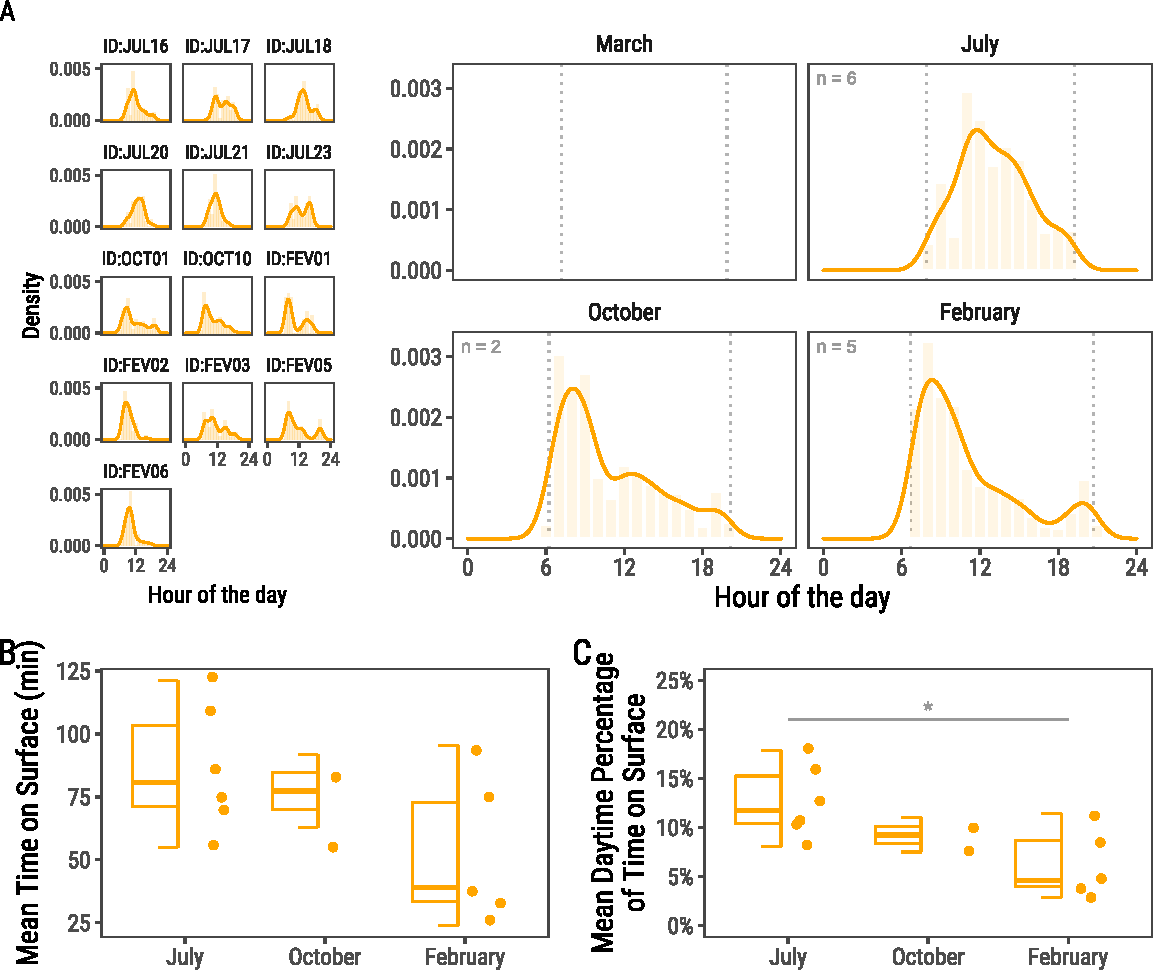
\includegraphics[width=1\linewidth]{tese_jefferson_files/figure-latex/plot-light-exposure-1} 

  }

  \caption{Tuco-tuco's daily patterns of surface emergence. (A) Density estimates of surface emergence. Solid lines indicate the Gaussian kernel density estimates. Light-colored bars shows observed surface emergence per hour. X-axis is hour of the day in Anillaco, La Rioja (UTC-3). Dotted vertical lines show time of civil twilights. (B) Mean time tuco-tucos spent on the surface per day. (C) Mean percentage of time on surface in relation to the daylength.}\label{fig:plot-light-exposure}
  \end{figure}
  \clearpage

  \hypertarget{general-activity}{%
  \subsection{General Activity}\label{general-activity}}

  Tuco-tuco's daily activity levels (24-hour average), measured by VeDBA, are significantly different across the year (ANOVA; F = 7.182, p \textless{} 0.01; Figure \ref{fig:vedba-boxplot}). Post hoc comparisons using Tukey-Kramer's Test shows significant group differences between July-October and July-February (p \textless{} 0.05). In both pairwise comparisons daily VeDBA levels in July are lower, showing a difference in means of 0.029 g in comparison to October and 0.019 g in comparison to February. In sum, daily VeDBA activity levels are lower in July in comparison to October and February (Fig \ref{fig:vedba-boxplot}).

  The daytime VeDBA (Light Phase Average) is also significantly different between months (ANOVA; F = 7.282, p \textless{} 0.001). Post hoc comparisons using Tukey-Kramer's Test shows a difference in mean of 0.035 between October-July only (p \textless{} 0.05). \newline
  \begin{figure}[H]

  {\centering 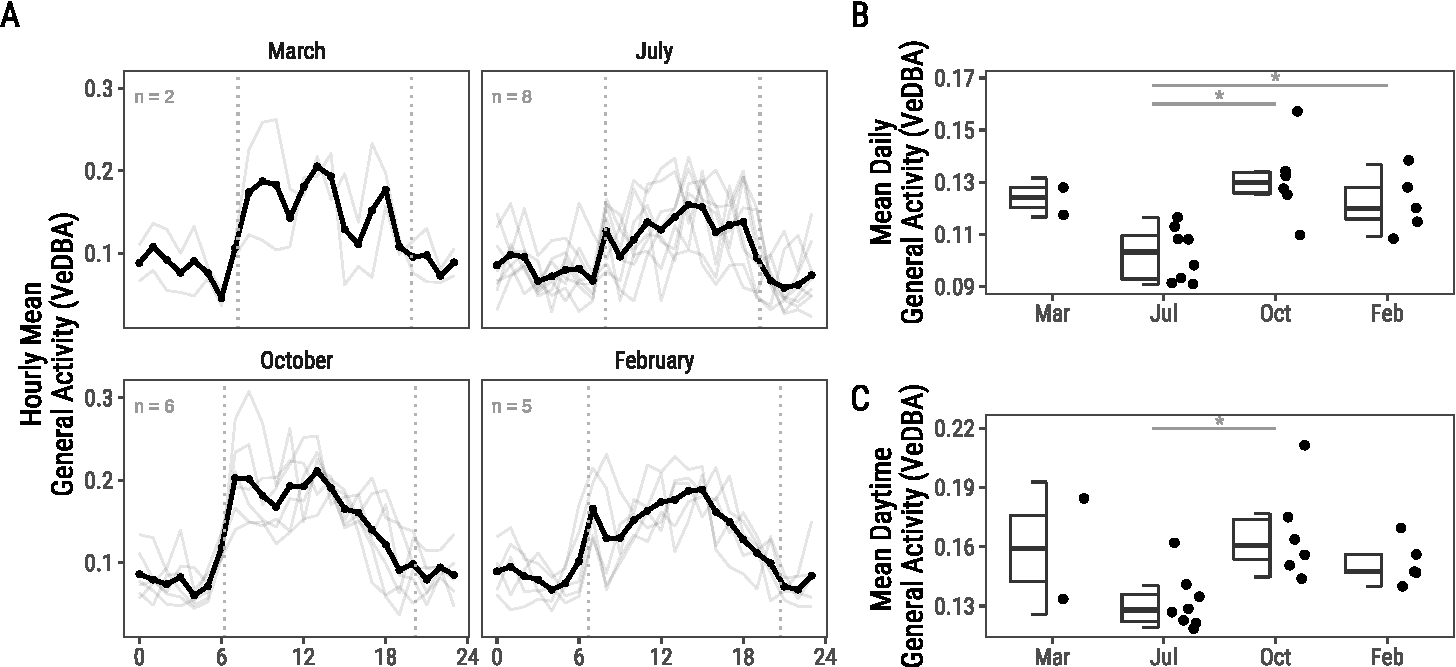
\includegraphics[width=1\linewidth]{tese_jefferson_files/figure-latex/vedba-boxplot-1} 

  }

  \caption{Tuco-tuco's Daily VeDBA levels. (A) VeDBA was binned by hour (0-23). Background lines show data for individual animals. Thick lines show mean hourly VeDBA. (B) Points show daily (24h) mean VeDBA for each animal. In July Tuco-tuco's exhibited lower Daily VeDBA than October and February. Dashed lines in Panel A shows time of civil dawn and dusk. Asterisks shows significant statistical difference between groups in an ANOVA followed by Tukey-Kramer's Test.}\label{fig:vedba-boxplot}
  \end{figure}
  \hypertarget{activity-state-classification}{%
  \subsection{Activity State Classification}\label{activity-state-classification}}

  We fitted two different HMMs to VeDBA data, one empty model, with no covariates, and a second one with \emph{`season'} as a covariate in the transition probability matrix. The second model was selected based on informational criterion (\(\Delta\)AIC \textgreater{} 2; REF Tabela AIC nos supps).

  The estimated state-dependent distributions are shown in Figure \ref{fig:hmm-plot}. We interpreted and labelled these states as `Rest,' `Medium intensity activity,' and `High intensity activity' corresponding to low, intermediate, and high VeDBA values respectively. The marginal distribution (Figure \ref{fig:hmm-plot}; dashed line) has a good correspondence to the empirical VeDBA distribution. A visual analysis of the Pseudo-residuals (Figure \ref{fig:appendix-residuals}) shows that the residuals deviate from the expected normal distribution, especially in the lower end values, and that there is still significant residual autocorrelation. Nevertheless, the overall fitting seems to be reasonable. The estimated state-dependent parameters are shown in the Appendix (Table \ref{tab:appendix-parameters}). \newline
  \begin{figure}[H]

  {\centering 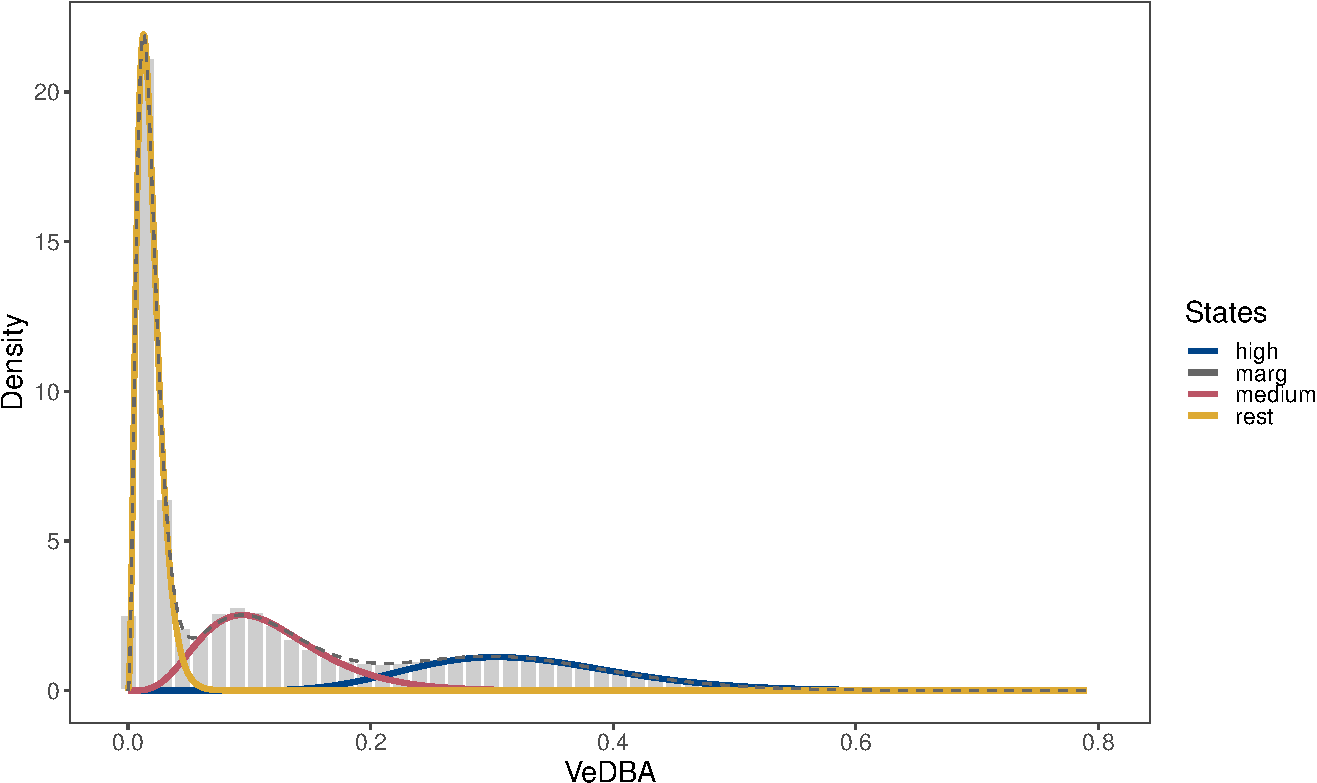
\includegraphics[width=1\linewidth]{tese_jefferson_files/figure-latex/hmm-plot-1} 

  }

  \caption{State-dependent distributions of the selected Hidden Markov model fitted to the VeDBA acceleration metric. Histogram, in grey, shows the Vectorial Dynamic Body Acceleration (VeDBA) from the data of 21 Anillaco's tuco-tuco. State-dependent gamma distributions are shown above the histograms. These distributions are weighted accordingly to the proportion of observations assigned to each state.}\label{fig:hmm-plot}
  \end{figure}
  With the state-labeled data we were able to dissociate and visualize the daily patterns of each different state. Actograms and time series plots show how the different states are related to the calculated VeDBA (Figure \ref{fig:actograms-results}). Visual analysis of diel rhythms in VeDBA and in the state-labelled data indicates the daily rhythm is more robust in the High Activity state in comparison to Medium Activity.

  However, despite being more concentrated during the daylight hours, High Activity episodes also occur sporadically during the night. Medium Activity, in turn, seems to be more spread throughout the day with no clear 24-hour rhythm. Individual Actograms for VeDBA and state-labelled data are presented in the Appendix (Figure \ref{fig:vedba-actograms}). \newline
  \begin{figure}[H]

  {\centering 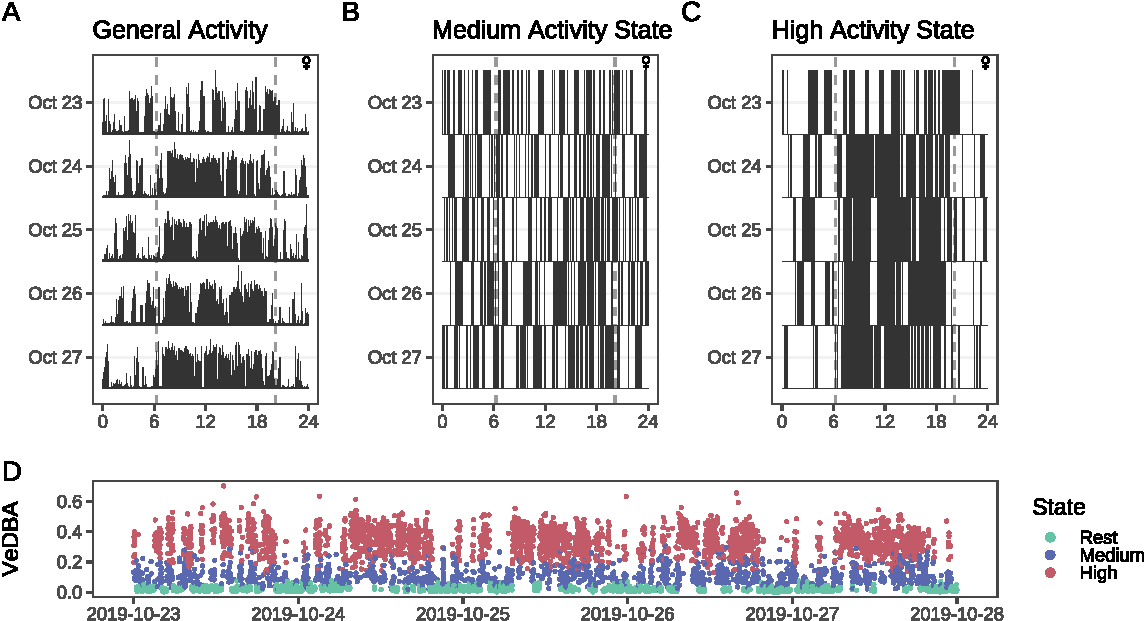
\includegraphics[width=1\linewidth]{tese_jefferson_files/figure-latex/actograms-results-1} 

  }

  \caption{Actograms and Time Series Plot of general activity, measured by VeDBA, and state-labelled data of a representative animal (ID:OCT09). The actograms shows daily patterns of VeDBA (A) and of Medium and High State occurrences (B and C). Medium Activity State shows no clear pattern of a daily rhythm. High Activity is spread throughout the day with a higher concentration during daylight hours. The time series (D) shows state-labelled VeDBA data. Dashed lines shows time of dawn and dusk.}\label{fig:actograms-results}
  \end{figure}
  \clearpage

  \hypertarget{daily-time-activity-budgets}{%
  \subsection{Daily Time-Activity Budgets}\label{daily-time-activity-budgets}}

  On average, tuco-tucos spent between 45-50\% of the 24 hours in the Rest state, with no statistical difference between the percentage of time spent resting between seasons (ANOVA; F = 1.93, p = 0.163). The remaining time is spent in an active state, either Medium or High Activity State.

  Tuco-tucos spent a variable percentage of their daily active time in one of the two active states, High or Medium, across seasons. Daily time spent in High Activity was lower in July (15.8\%) and higher in October (29.4\%). In contrast, daily time spent in a Medium Activity State was higher in July (34.1\%) and lower in October (24.8\%). There is a significant difference in the percentage of time spent in Medium (Figure \ref{fig:plot-time-state}; ANOVA: F = 4.457, p = 0.0175) and High Activity State across seasons (Figure \ref{fig:plot-time-state}; ANOVA: F = 13.62, p = \textless{} 0.001). Tukey's post hoc test shows that the mean percentage of time spent in the Medium Activity State is 9\% lower in October than in July (p = 0.01). For the High Activity State, pairwise Tukey's test shows a significant difference between October-July (p \textless{} 0.001) and February-July (p \textless{} 0.01). In comparison to July the mean daily percentage of time spent in a High Activity State is 13\% higher in October and 8\% higher in February (Figure \ref{fig:plot-time-state}).
  \begin{figure}

  {\centering 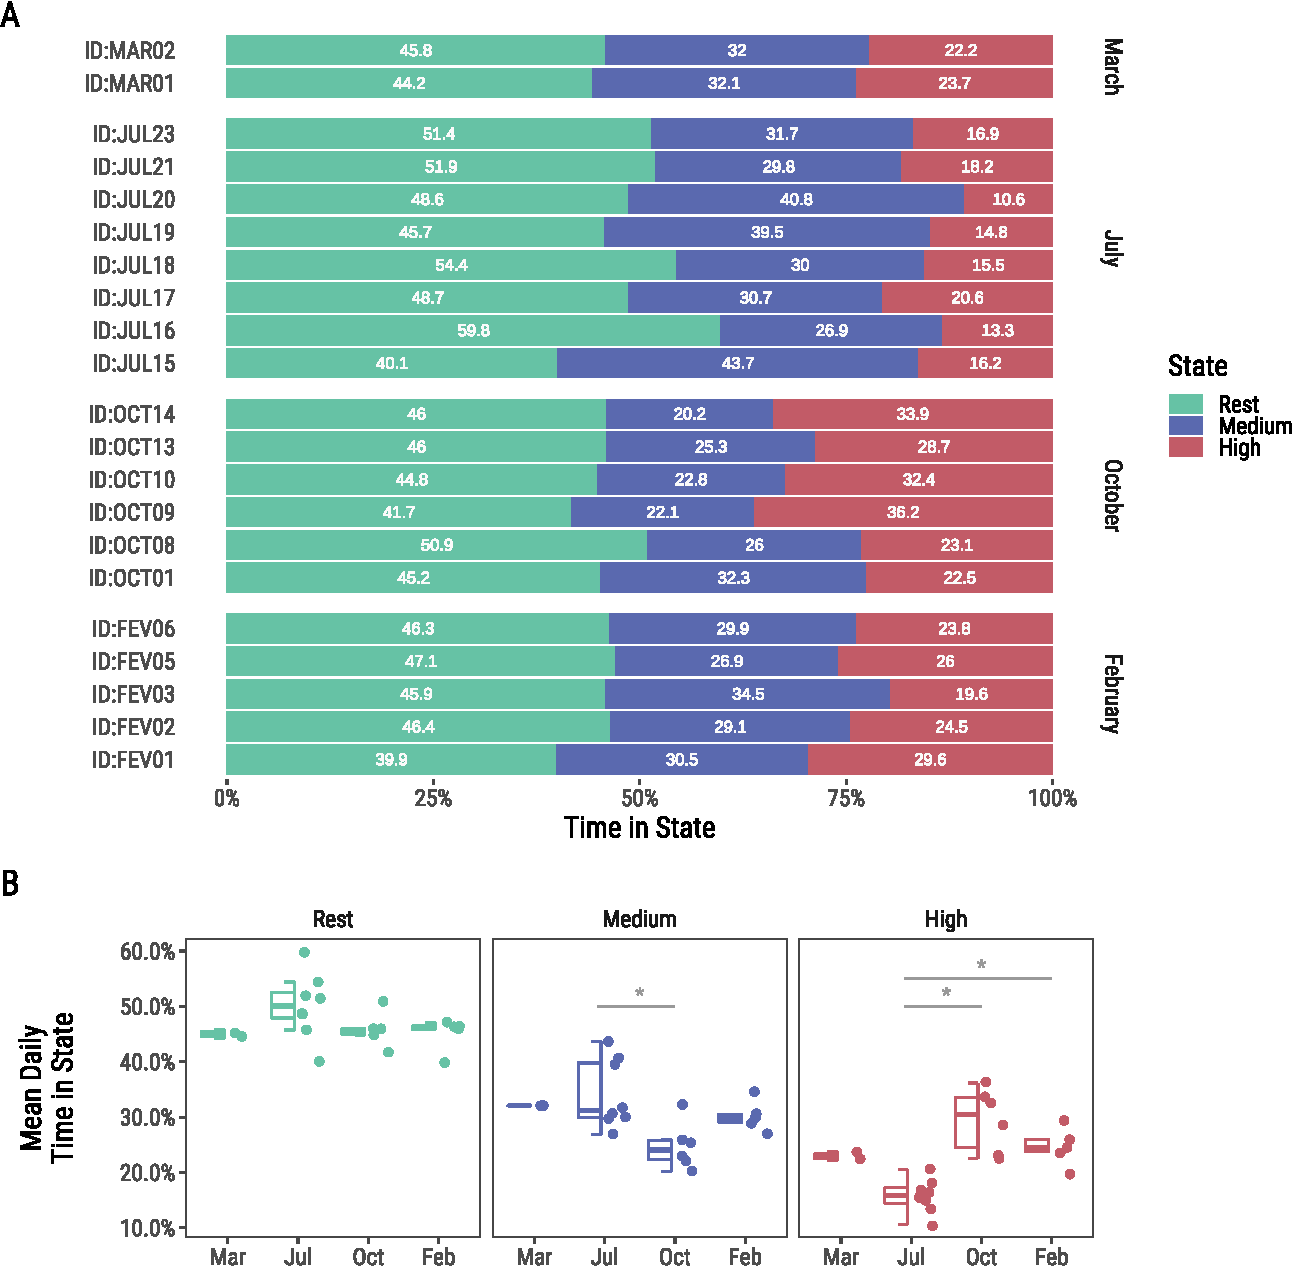
\includegraphics[width=1\linewidth]{tese_jefferson_files/figure-latex/plot-time-state-1} 

  }

  \caption{Daily time-activity budgets for the behavioral states. (A) Percentage of time spent in each behavioral state per animal. (B) Boxplot and individual points of the distribution of the mean percentage of time spent in each behavioral state. Asteriscs shows statistical significant pairwise comparison between Months. The mean percentage of time spent in the High Activity State is lower in July in comparison to October and February. The mean percentage of time spent in the Medium Activity State, however, is higher in July in comparison with October.}\label{fig:plot-time-state}
  \end{figure}
  \newpage

  \hypertarget{daily-activity-patterns}{%
  \subsection{Daily Activity Patterns}\label{daily-activity-patterns}}

  Daily activity patterns for each behavioral state are shown in Figure \ref{fig:plot-patterns}. These plots show that, qualitatively, the timing of occurrence of High Activity and Light Exposure episodes follow a diurnal pattern. Medium Activity, however, is spread out along the 24h and do not follow a daily (24-hour) rhythm. It is important to note that the timing of peak occurrence of High Activity behavior does not appear to change dramatically along the year. In all four Months the peak of High Activity is around 14:00.
  \begin{itemize}
  \tightlist
  \item
    REF calculate peak
  \item
    REF adicionar linha do meio dia solar
  \end{itemize}
  \newpage
  \begin{figure}

  {\centering 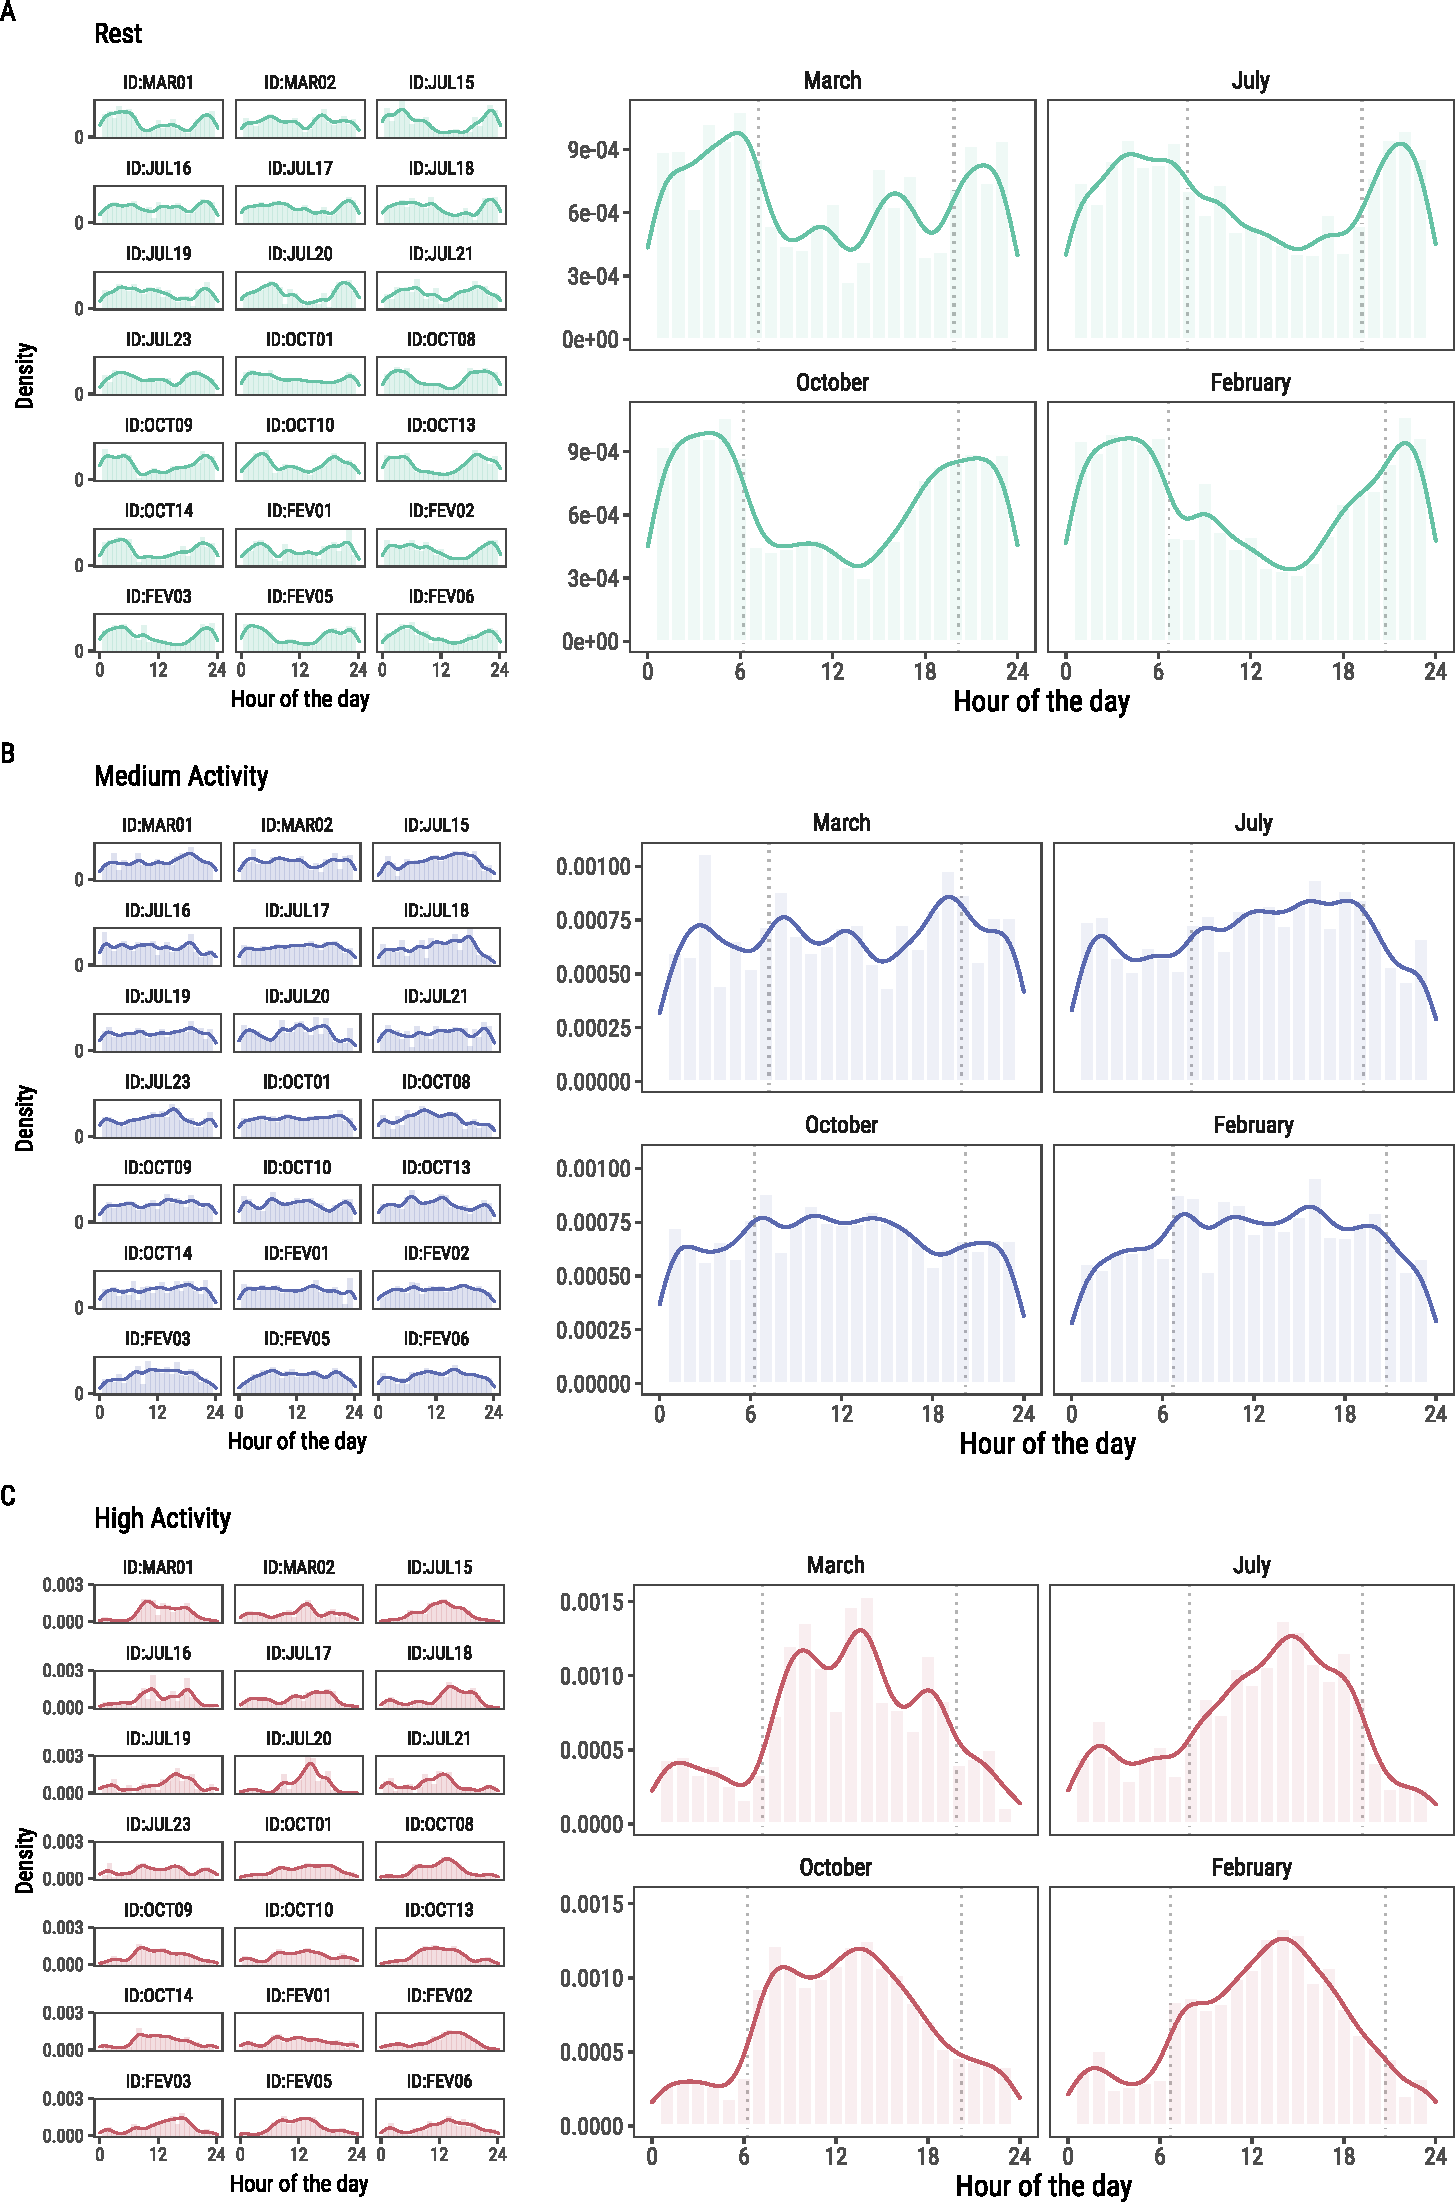
\includegraphics[width=0.95\linewidth]{tese_jefferson_files/figure-latex/plot-patterns-1} 

  }

  \caption{Density estimates of daily activity patterns of tuco-tucos' behavioral states. Solid lines indicate the Gaussian kernel density estimates. Light-colored bars show observed distribution of each behavioral state occurrence. The x-axis is hour of the day in Anillaco, La Rioja (UTC-3). Dotted vertical lines show time of civil twilights. (A) High Activity State shows a diurnal pattern independent of the time of the year. (B) Medium Activity State shows no daily pattern. (C) Daily pattern of light exposure changes according to the season.}\label{fig:plot-patterns}
  \end{figure}
  \clearpage

  \hypertarget{aboveground-activity}{%
  \subsection{Aboveground Activity}\label{aboveground-activity}}

  Outside of their tunnels, when exposed to light, tuco-tucos are mostly in a active state, either high or medium state (Fig. \ref{fig:aboveground-activity}). The percentage of the high activity state that occurs on the surface is higher than the other activity states. The mean percentage of the high state that occurs aboveground is 0.15, whether for the medium state the mean is 0.05. Rest, in contrast, is the behavioral state that happens the least on the surface with a mean percentage of 0.01.\newline
  \begin{itemize}
  \tightlist
  \item
    aqui ainda falta um teste. Precisa ser um não parametrico ou test-t dois a dois. O ANOVA não cabe nesses dados.
  \end{itemize}
  \begin{figure}[H]

  {\centering 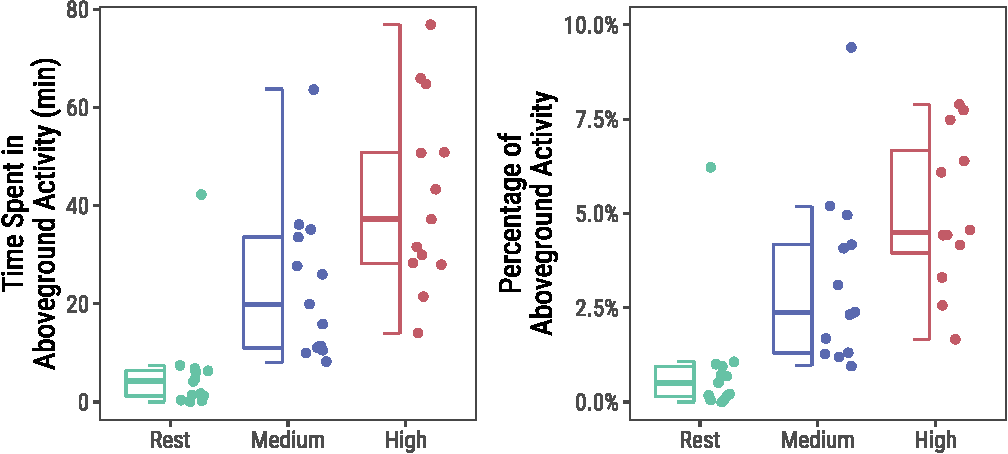
\includegraphics[width=1\linewidth]{tese_jefferson_files/figure-latex/aboveground-activity-1} 

  }

  \caption{Distribution of the percentages of each activity state that happens aboveground during daytime.}\label{fig:aboveground-activity}
  \end{figure}
  \newpage

  \hypertarget{diurnality}{%
  \subsection{Diurnality}\label{diurnality}}

  High Activity State is predominately diurnal (DI \textgreater{} 0.5). The average diurnality for the High Activity State is higher than 0.7 for all seasons. The Medium Activity State, however, has a diurnality index that ranges from 0.5 in March to 0.56 in July and February. The Rest State is predominantly nocturnal with Diurnality lower than 0.38 in all seasons. There is no statistical difference between seasons (ANOVA; p \textgreater{} 0.2 for all states; Figure \ref{fig:diurnality-plot}). \newline
  \begin{figure}[H]

  {\centering 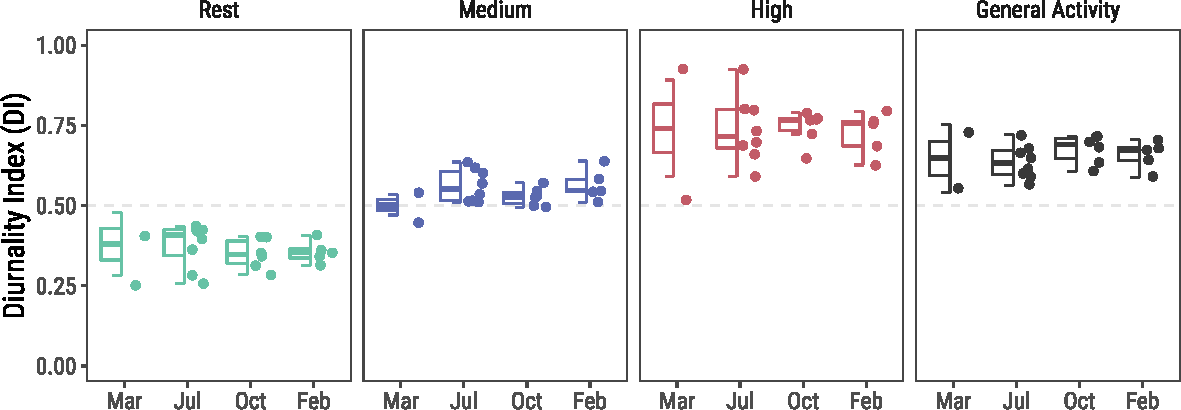
\includegraphics[width=1\linewidth]{tese_jefferson_files/figure-latex/diurnality-plot-1} 

  }

  \caption{Distribution of calculated diurnality index (DI). Between labelled states, only the High Activity State is predominantly diurnal, with diurnality greater than 0.7 across all season. General activity, measured by the unlabelled VeDBA, is also predominantly diurnal, }\label{fig:diurnality-plot}
  \end{figure}
  \newpage

  \hypertarget{circadian-rhythmicity}{%
  \subsection{Circadian Rhythmicity}\label{circadian-rhythmicity}}

  Circadian rhythms are present in all states as seen in the visual analysis of the autocorrelation plots (REF APPENDIX - plotar ACFs individuais). The percentage of animals classified as rhythmic is higher for the high activity state, where a total of 18 animals were classified as rhythmic (85.7\%). In contrast, the medium activity state had, in total, 11 animals (52.4\%) classified as rhythmic.

  We calculated the RI only for animals classified as rhythmic (Figure \ref{fig:plot-ri-and-period}A). It is important to note that animals classified as arrhythmic were excluded from this analysis, which is why there is a different number of samples between each category. Nonetheless, the Medium Activity State is significantly different from the other states and VeDBA (Figure \ref{fig:plot-ri-and-period}A; ANOVA; p \textless{} 0.05). We did not test for differences between seasons (See Methods).

  Lastly, we used Lomb-Scargle periodograms to estimate the periodicity of each state (Figure \ref{fig:plot-ri-and-period}B). All estimated periods, independent of state, were in the 24-hour range. The high activity state has a mean period ± standard deviation of 23.87h ± 0.34. The medium activity state has a mean period of 23.91h ± 1.22.

  We also estimated RI and periodicity for VeDBA. In comparison with state-labelled data VeDBA analysis are more similar to the high activity state. The number of animals classified as rhythmic based on the autocorrelation plot is similar between VeDBA and high activity state data. The distribution of RI shows no difference between High state and VeDBA (Figure \ref{fig:plot-ri-and-period} A). For VeDBA the mean estimated period was 23.91h ± 0.31.
  \begin{figure}[H]

  {\centering 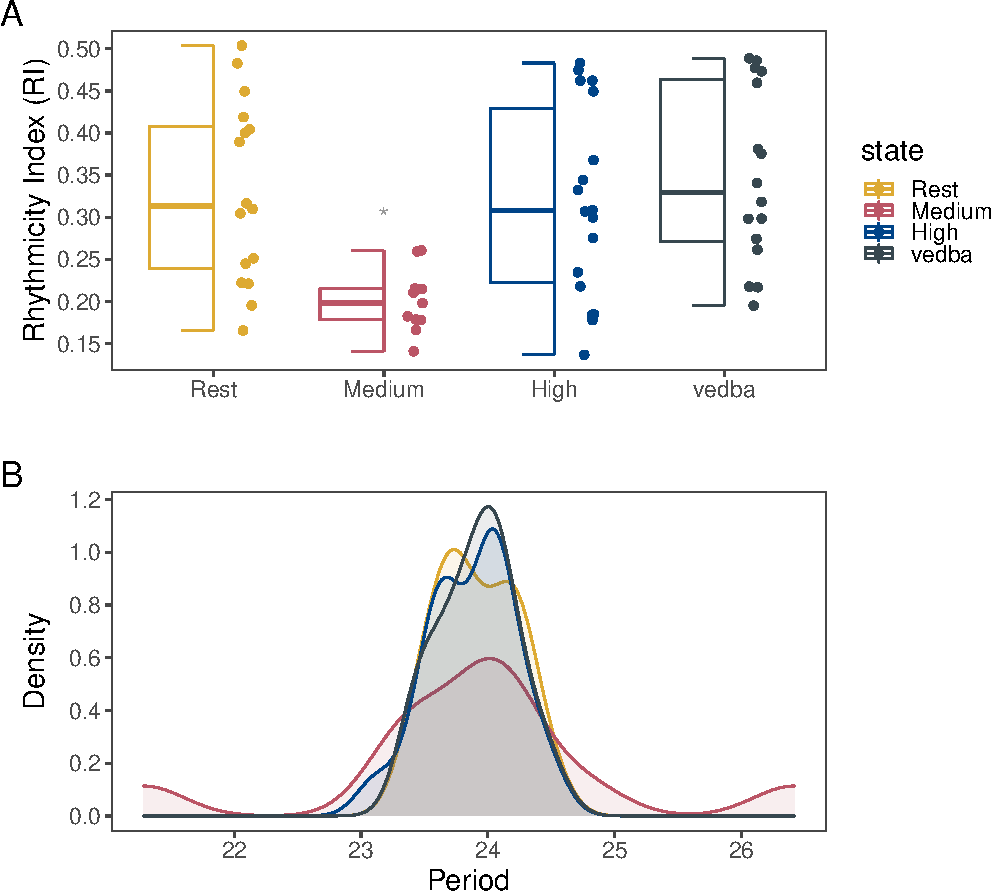
\includegraphics[width=1\linewidth]{tese_jefferson_files/figure-latex/plot-ri-and-period-1} 

  }

  \caption{Distribution of Rhythmicity Index for state-labelled data and VeDBA. The distribution of the Medium State is statistically different from all other states and VeDBA. Graphs shows half boxplots and individual data}\label{fig:plot-ri-and-period}
  \end{figure}
  \newpage

  \hypertarget{discussion}{%
  \section{Discussion}\label{discussion}}
  \begin{itemize}
  \item
    mencionar que tudo que é medido foi a primeira vez em vida livre
  \item
    Optamos pelo tipo de modelos mais simples com outras a analises a posteriori. Existem outros métodos interessantes Patterson 2009. Extensions to out model could include (\ldots)
    \begin{itemize}
    \tightlist
    \item
      selecionamos os fatores mais relevantes baseados nas analises exploratorias
    \end{itemize}
  \item
    limitações dos dados de lightlogger: não sabemos se os picos podem se extender durante a noite tbm.
  \item
    discutir as semelhancas entre arena e freeliving
    \begin{itemize}
    \tightlist
    \item
      o padrão é igual, explicar o que foi visto nas arenas
    \end{itemize}
  \item
    diferença ritmicidade vedba vs estados na ritmicidade
  \item
    falar que nem sempre o HMM é ideal para ritmicidade e diurnalidade
  \item
    uma boa mensagem para deixar pro futuro
  \item
    reler artigo catemeralidade
    \begin{itemize}
    \item
      nesse artigo foi percebido varios bouts de atividades
    \item
      tamiris: while not on the wheel they are doing different things
      \begin{itemize}
      \tightlist
      \item
        não podemos assumir que quando nao está na roda ele está parado
      \item
        erkert artigo + voles lehmann (trabalhos de catemeralidade)
      \item
        esse ponto é essencial para conectar com o que o HMM fez
      \item
        HMM trouxe a tona outros ritmos presentes ao longo de todo dia + o componente circadiano que tbm vemos na roda, p.e.
      \item
        tbm falar que não era possível medir -\textgreater{} tecnologias diferentes.
      \end{itemize}
    \end{itemize}
  \item
    Deixar os eixos como Atividade Geral (VeDBA)
    \begin{itemize}
    \tightlist
    \item
      colocar apenas na legenda que atividade geral é medida pelo VeDBA
    \end{itemize}
  \item
    Erkert, H.G.; Cramer B. 2006. Chronobiological background to cathemerality: circadian rhythms in Eulemur fulvus albifrons (Prosimili) and Aotus azarai boliviensis (Anthropoidea). Folia Primatologica 77: 87--113.
  \item
    lehmann
  \item
    A atividade ``catemera'' não era prevista então isso é uma coisa interessante
    \begin{itemize}
    \tightlist
    \item
      falar que é novo e interessante
    \item
      tudo isso foi medido pq fomos ao campo
    \item
      ``qual a relacao entre o circadiano e os ultradianos?''
    \end{itemize}
  \end{itemize}
  \begin{center}\rule{0.5\linewidth}{0.5pt}\end{center}
  \begin{itemize}
  \item
    os resultados do indice de ritmicidade devem ser interpretados com cuidado já que existe diferença na classificação dos animais em primeiro lugar.
    \begin{itemize}
    \tightlist
    \item
      Isso principalmente na hora de interpretar o grafico de boxplot dos RI, entre HIGH e VEDBA.
    \end{itemize}
  \end{itemize}
  \appendix \# Apêndice \{-\}

  \hypertarget{anillacos-plant-community}{%
  \chapter{Anillaco's Plant Community}\label{anillacos-plant-community}}

  Following methods similar to (\protect\hyperlink{ref-aranda-rickert2014}{Aranda-Rickert, Diez, and Marazzi 2014}) a non-extensive survey of the plant community was done in May 2019. Three perpendicular 50m transects were defined near the study site (COORDINATES). A point-intercept method was used to record plant species present in the transects, species right below the sampling points were registered in the data. Sampling points were defined every 1m along the 50m transects. Plant species were identified in the field by a Botanist, except for a few members of the Poaceae family.

  The results for the plant survey is in line with what has been described in the literature for the region (\protect\hyperlink{ref-abraham2009}{Abraham et al. 2009}; \protect\hyperlink{ref-aranda-rickert2014}{Aranda-Rickert, Diez, and Marazzi 2014}; \protect\hyperlink{ref-fracchia2011}{Fracchia et al. 2011}). The results show a dominance of Zygolhyllaceae, Poaceae and Fabaceae families. The relative frequency of plant families and species recorded in the area are shown in the graphs below (Fig. \ref{fig:appendix-plants}).
  \begin{figure}

  {\centering 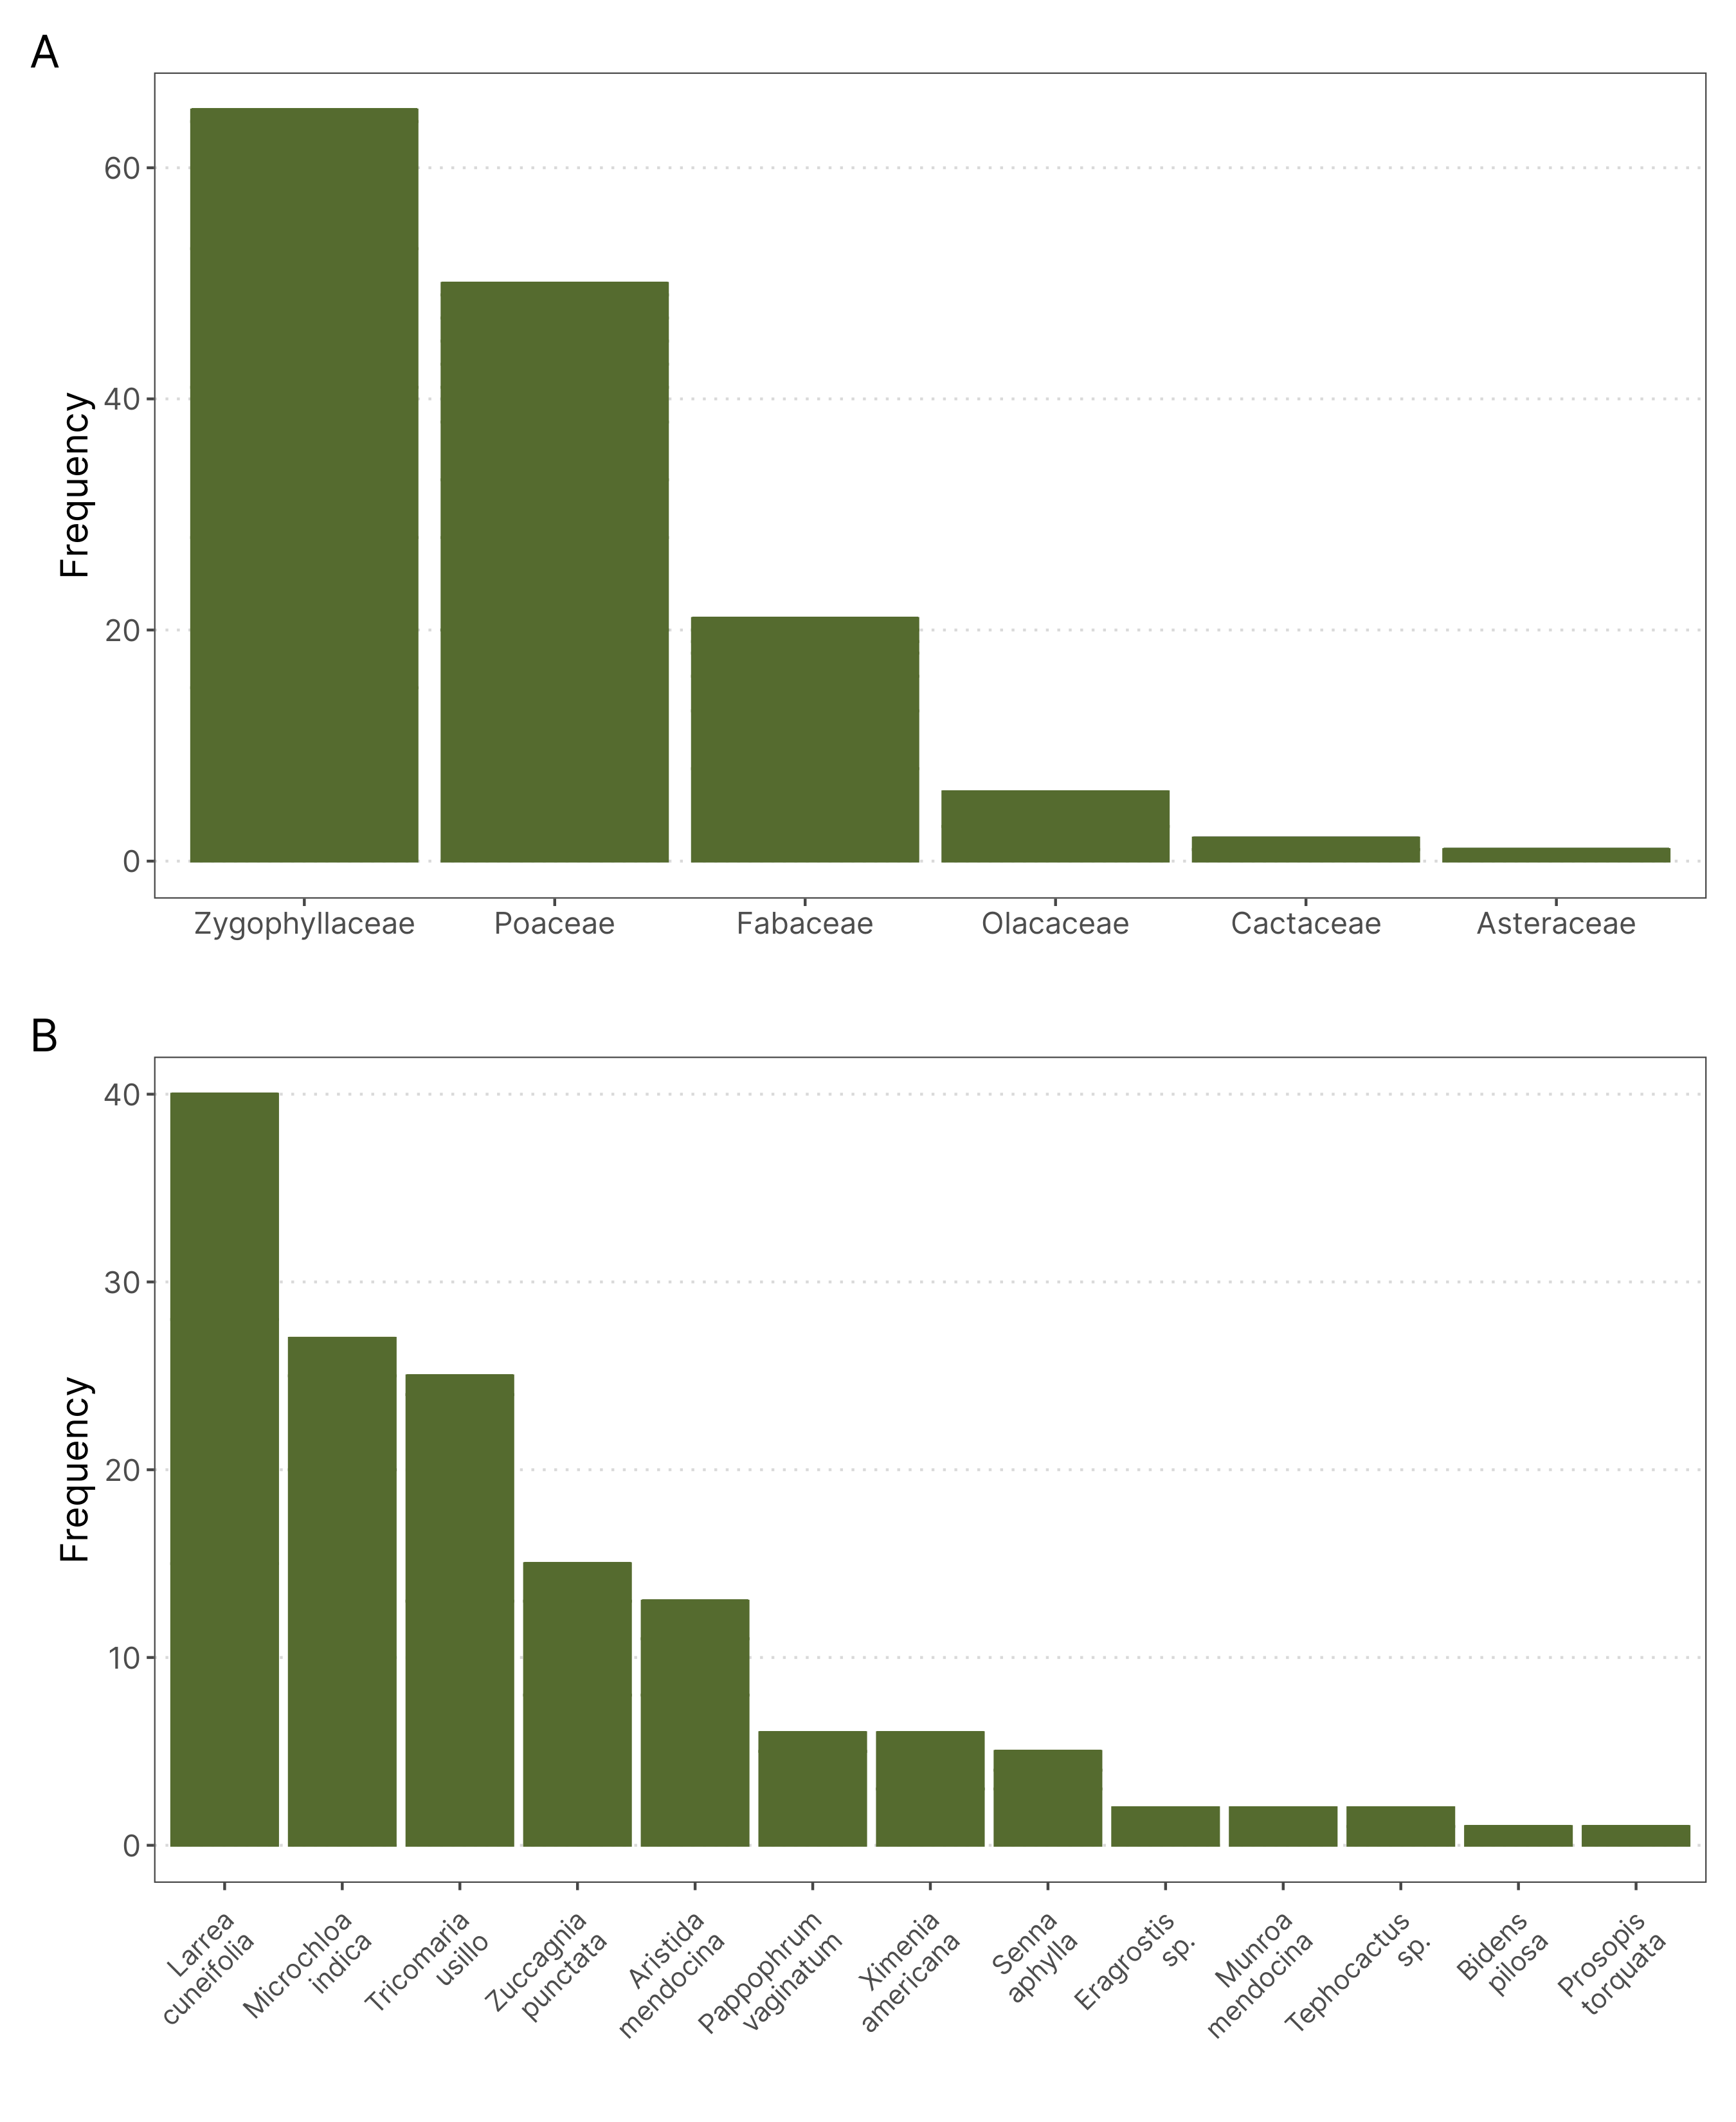
\includegraphics[width=1\linewidth]{../04_figures/appendix/plot_plants} 

  }

  \caption{Relative frequency of plants family (A) and species (B) in three transects near the Study Site. The plant community is dominated by members of the Zygolhyllaceae, Poaceae and Fabaceae families and is in accordance with what has been described in the literature. (n = 145)}\label{fig:appendix-plants}
  \end{figure}
  \hypertarget{anillacos-weather}{%
  \chapter{Anillaco's Weather}\label{anillacos-weather}}
  \begin{figure}

  {\centering 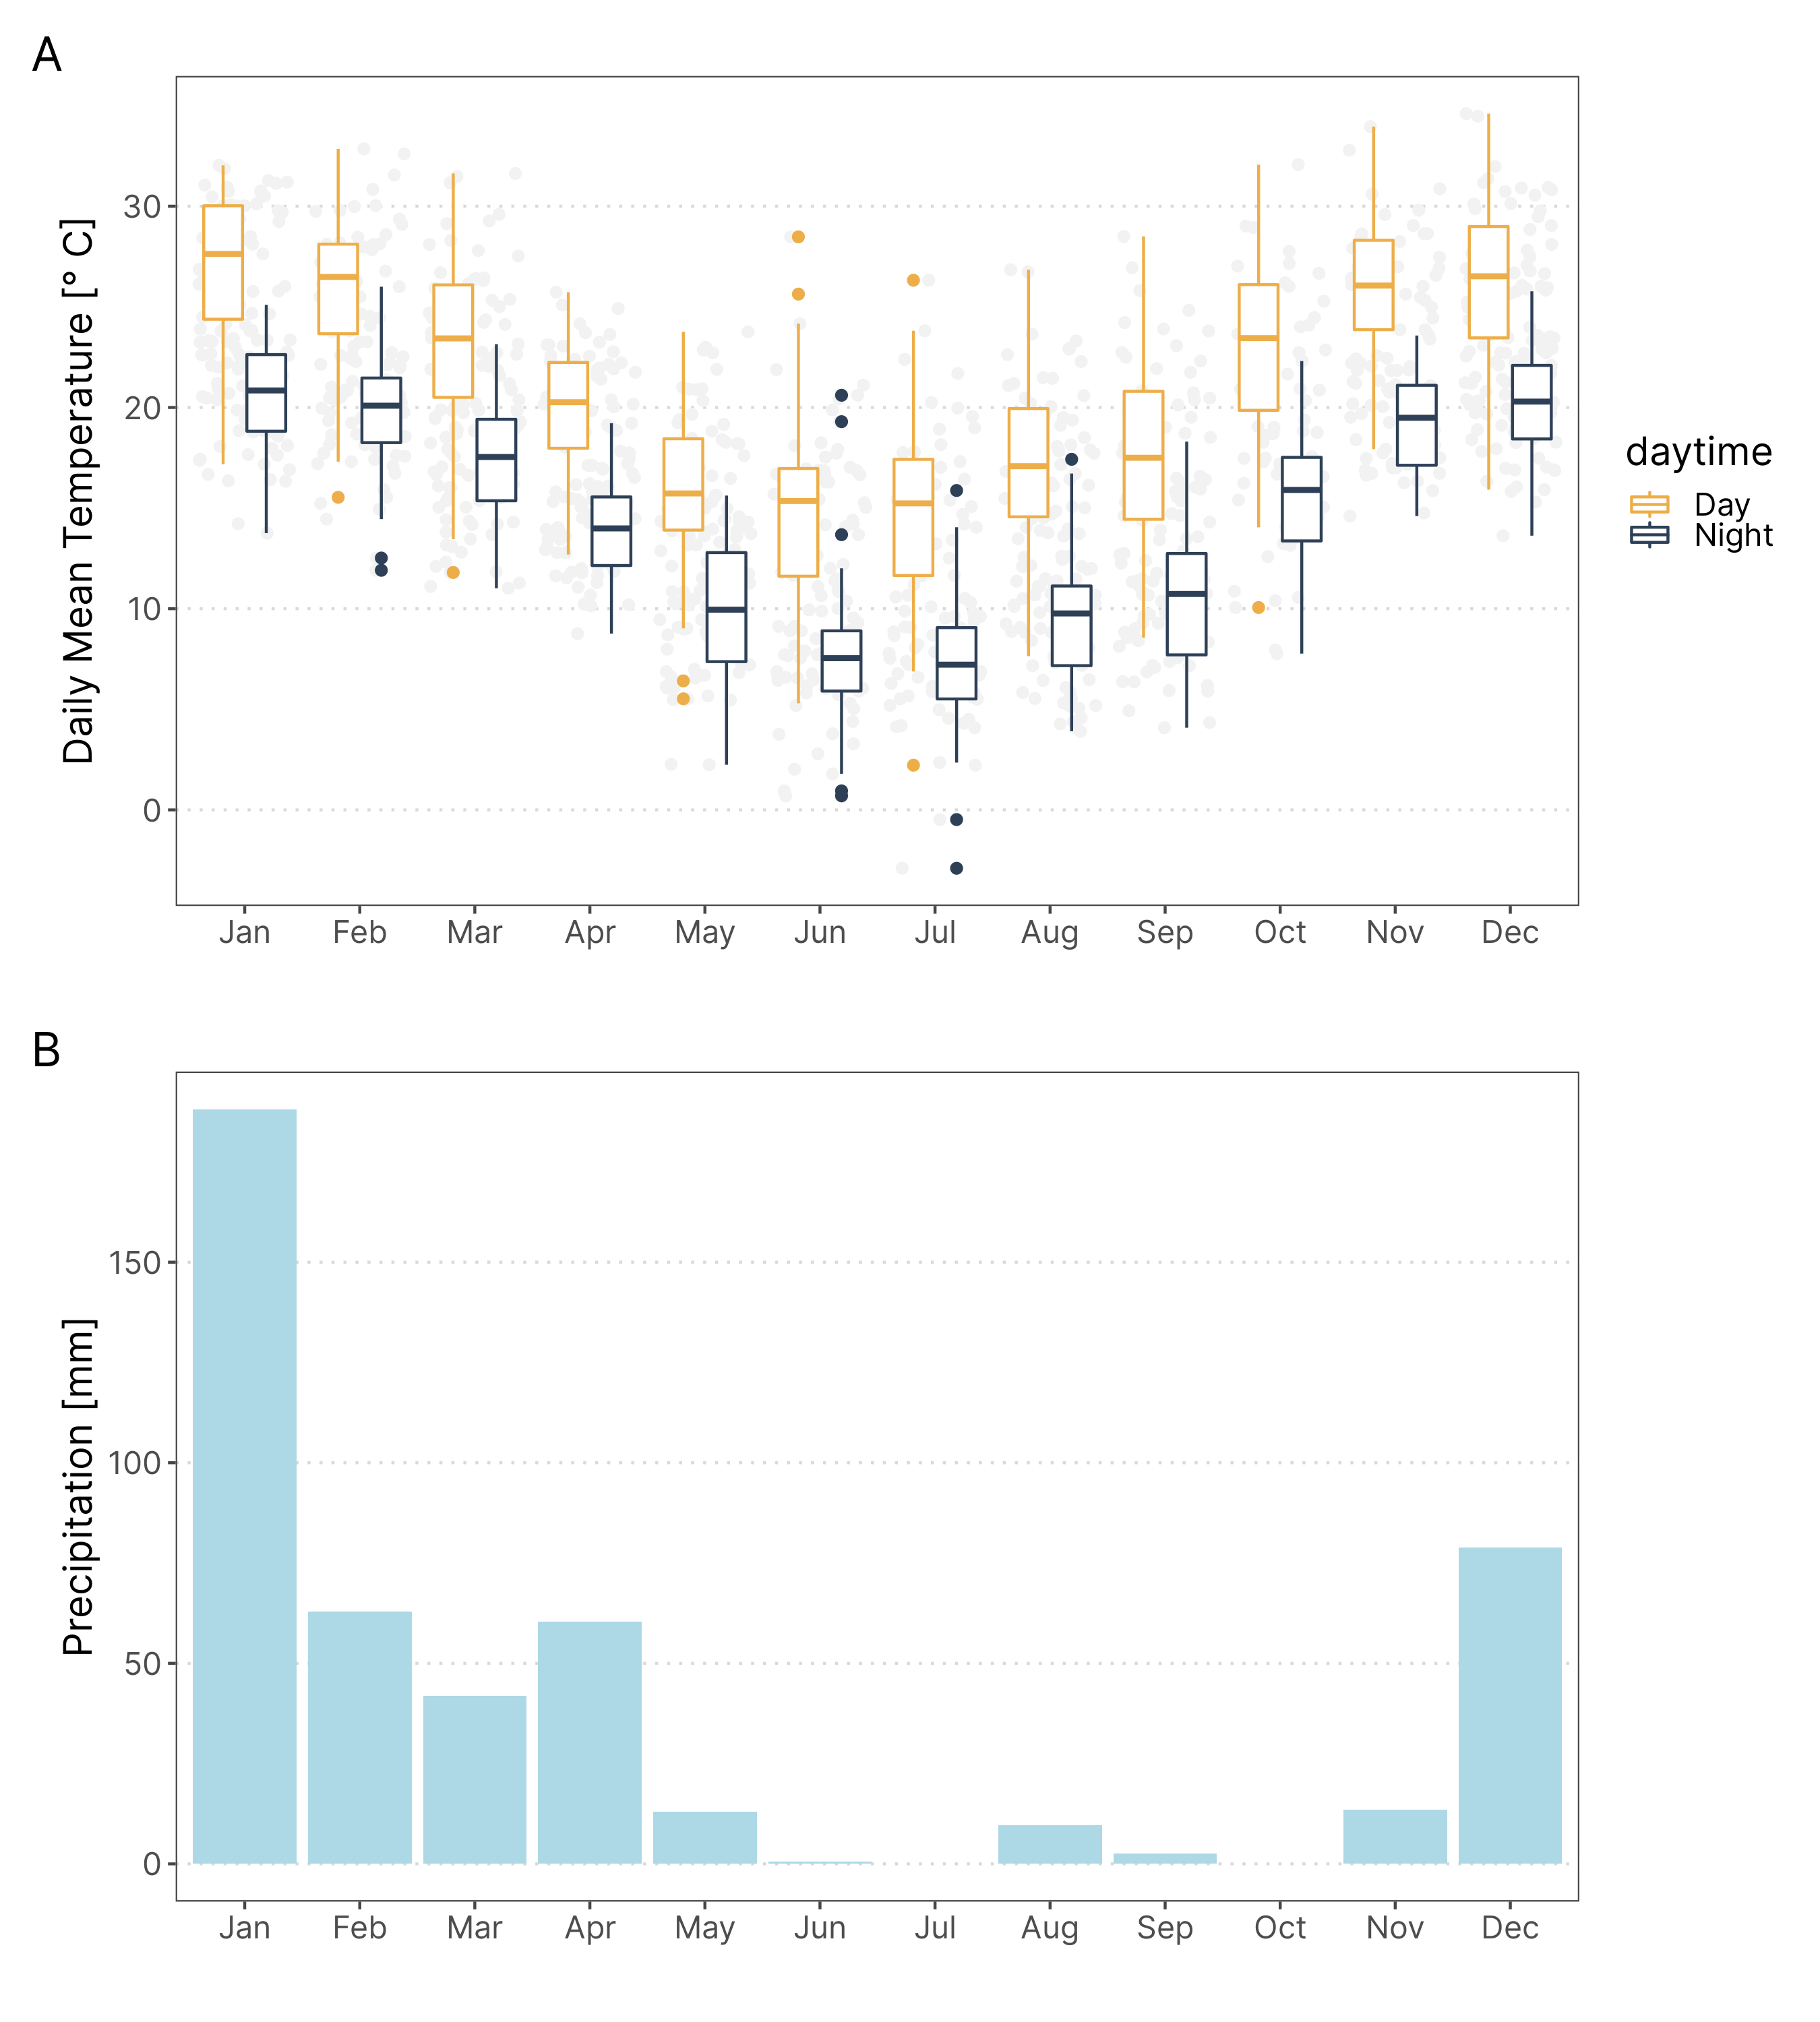
\includegraphics[width=1\linewidth]{../04_figures/appendix/plot_weather} 

  }

  \caption{Temperature  and Rainfall yearly trends in Anillaco, Argentina. Data was collected in the years 2017 and 2019 from a weather Station (Vantage Pro 2, Davis Instuments. USA.) maintened in CRILAR, aproximately 5km away from the study site.}\label{fig:appendix-weather}
  \end{figure}
  \hypertarget{anillacos-yearly-daylength-changes}{%
  \chapter{Anillaco's Yearly Daylength Changes}\label{anillacos-yearly-daylength-changes}}
  \begin{itemize}
  \tightlist
  \item
    Adicionar tabela com duração do dia nas datas de coleta
  \end{itemize}
  \begin{figure}

  {\centering 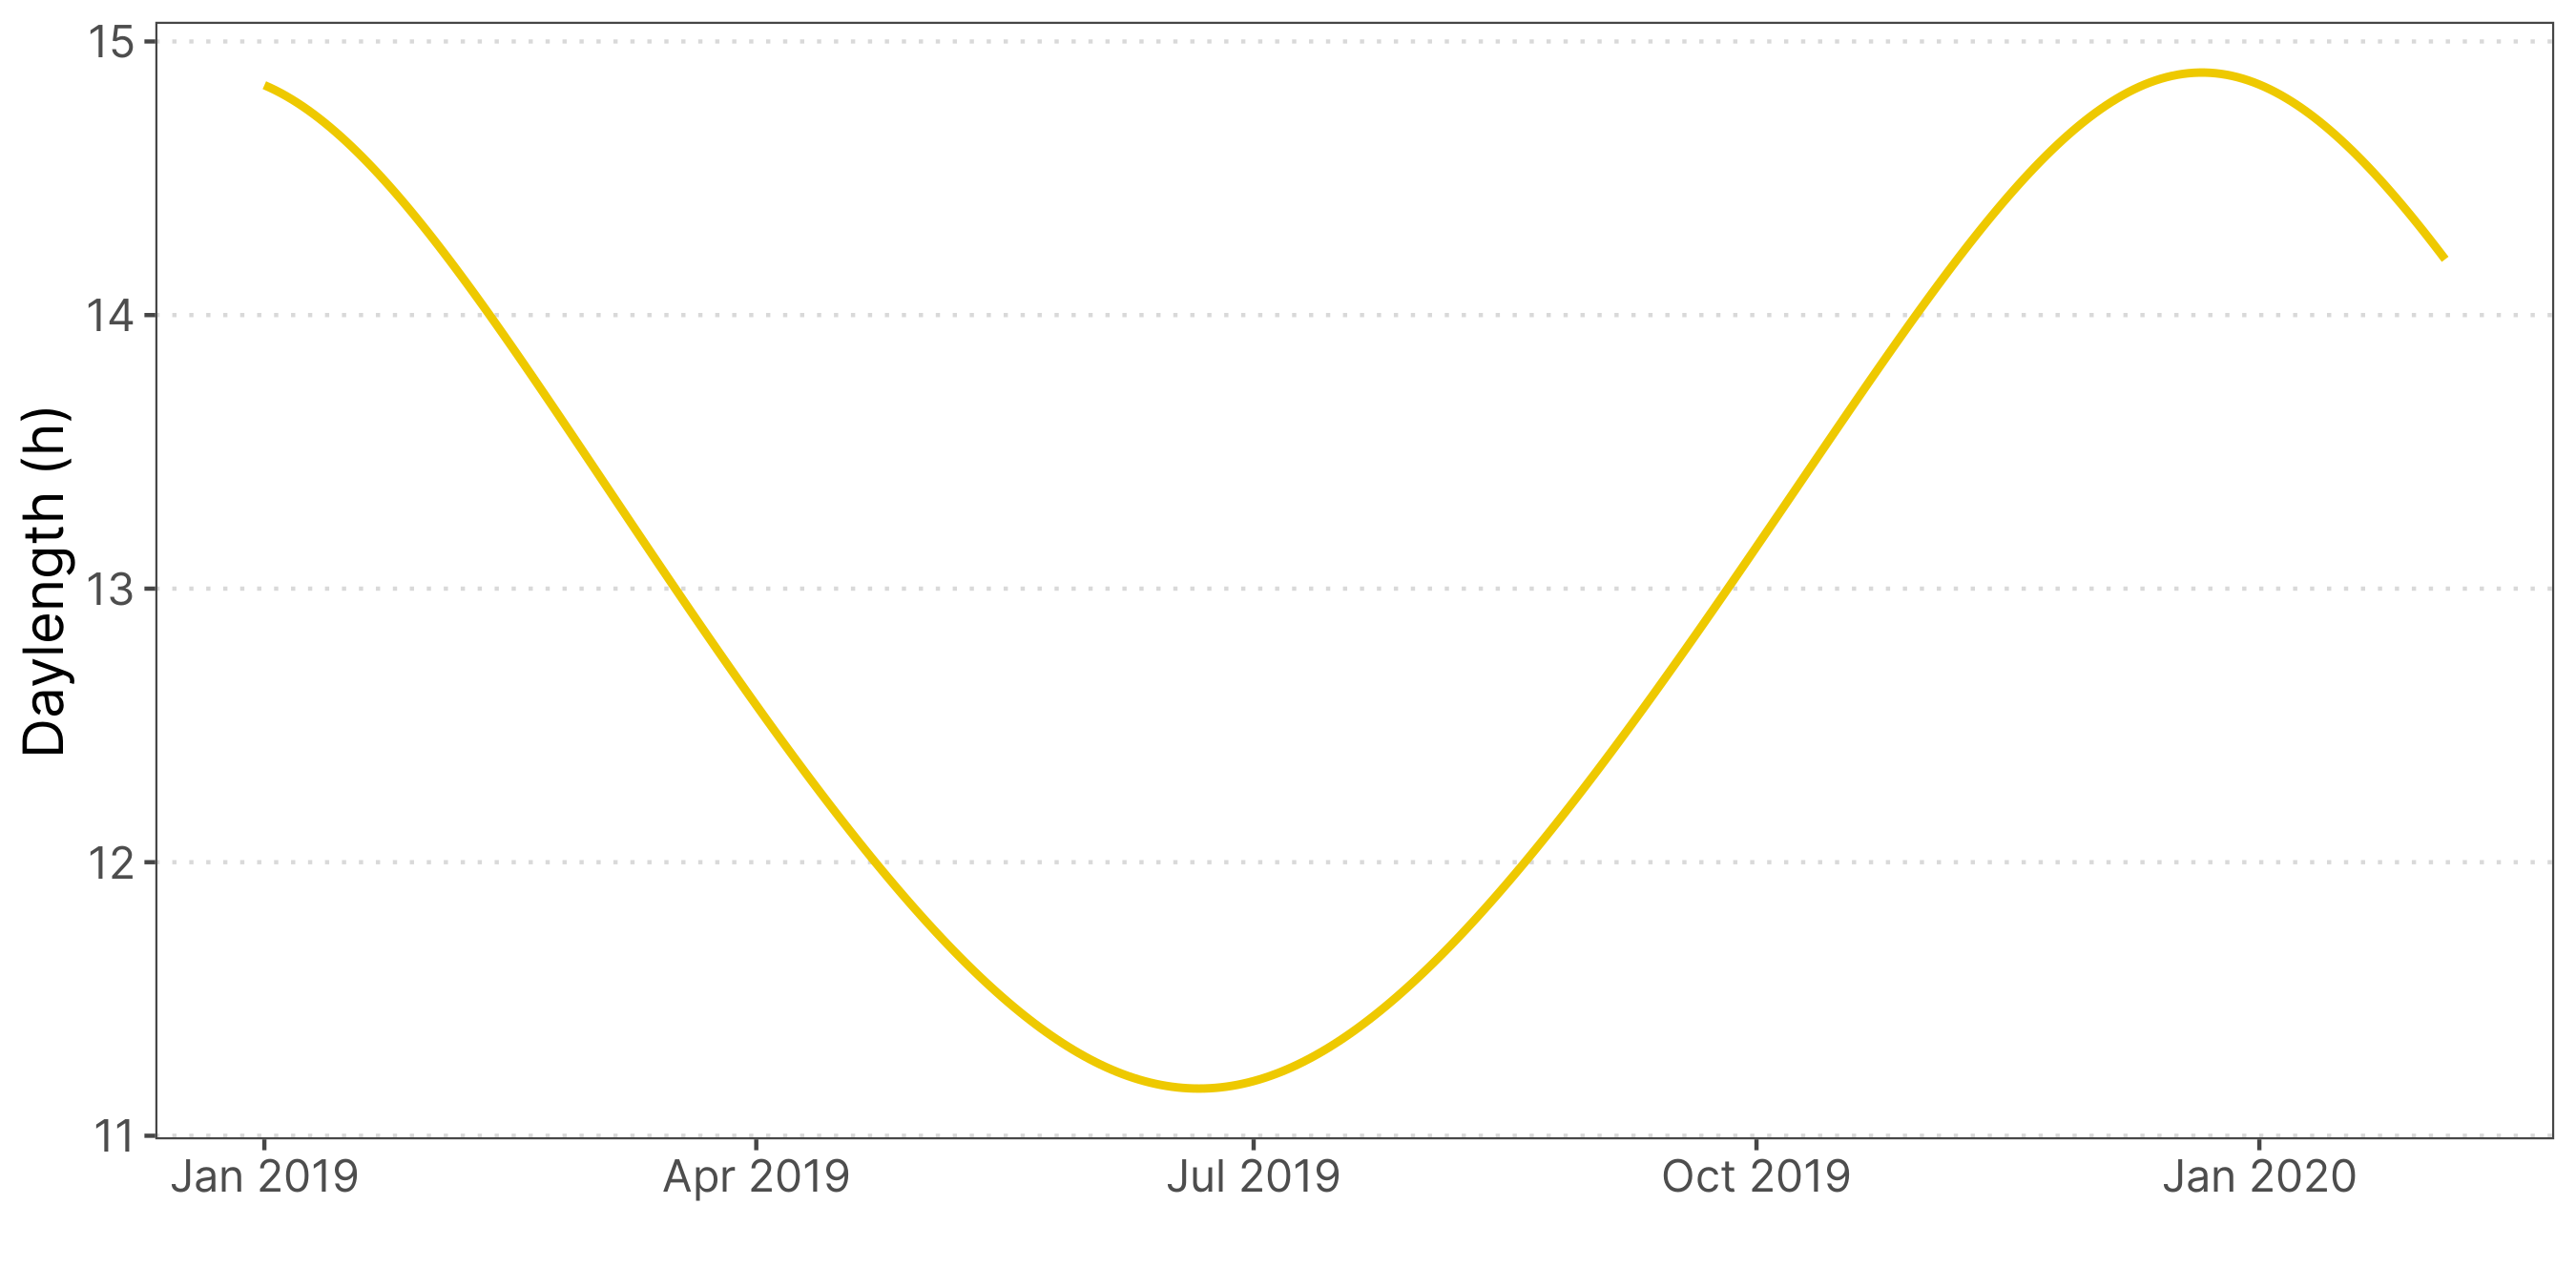
\includegraphics[width=1\linewidth]{../04_figures/appendix/plot_daylength} 

  }

  \caption{Changes in daytime changes across the year in Anillaco, La Rioja. Maximum duration of daytime, during summer, is 14 hours and 53 minutes. Mininum duration of daytime, during winter, is 11 hours and 10 minutes.}\label{fig:appendix-daylenght}
  \end{figure}
  \hypertarget{static-acceleration-smooth-window-assessment}{%
  \chapter{Static Acceleration Smooth Window Assessment}\label{static-acceleration-smooth-window-assessment}}
  \begin{center}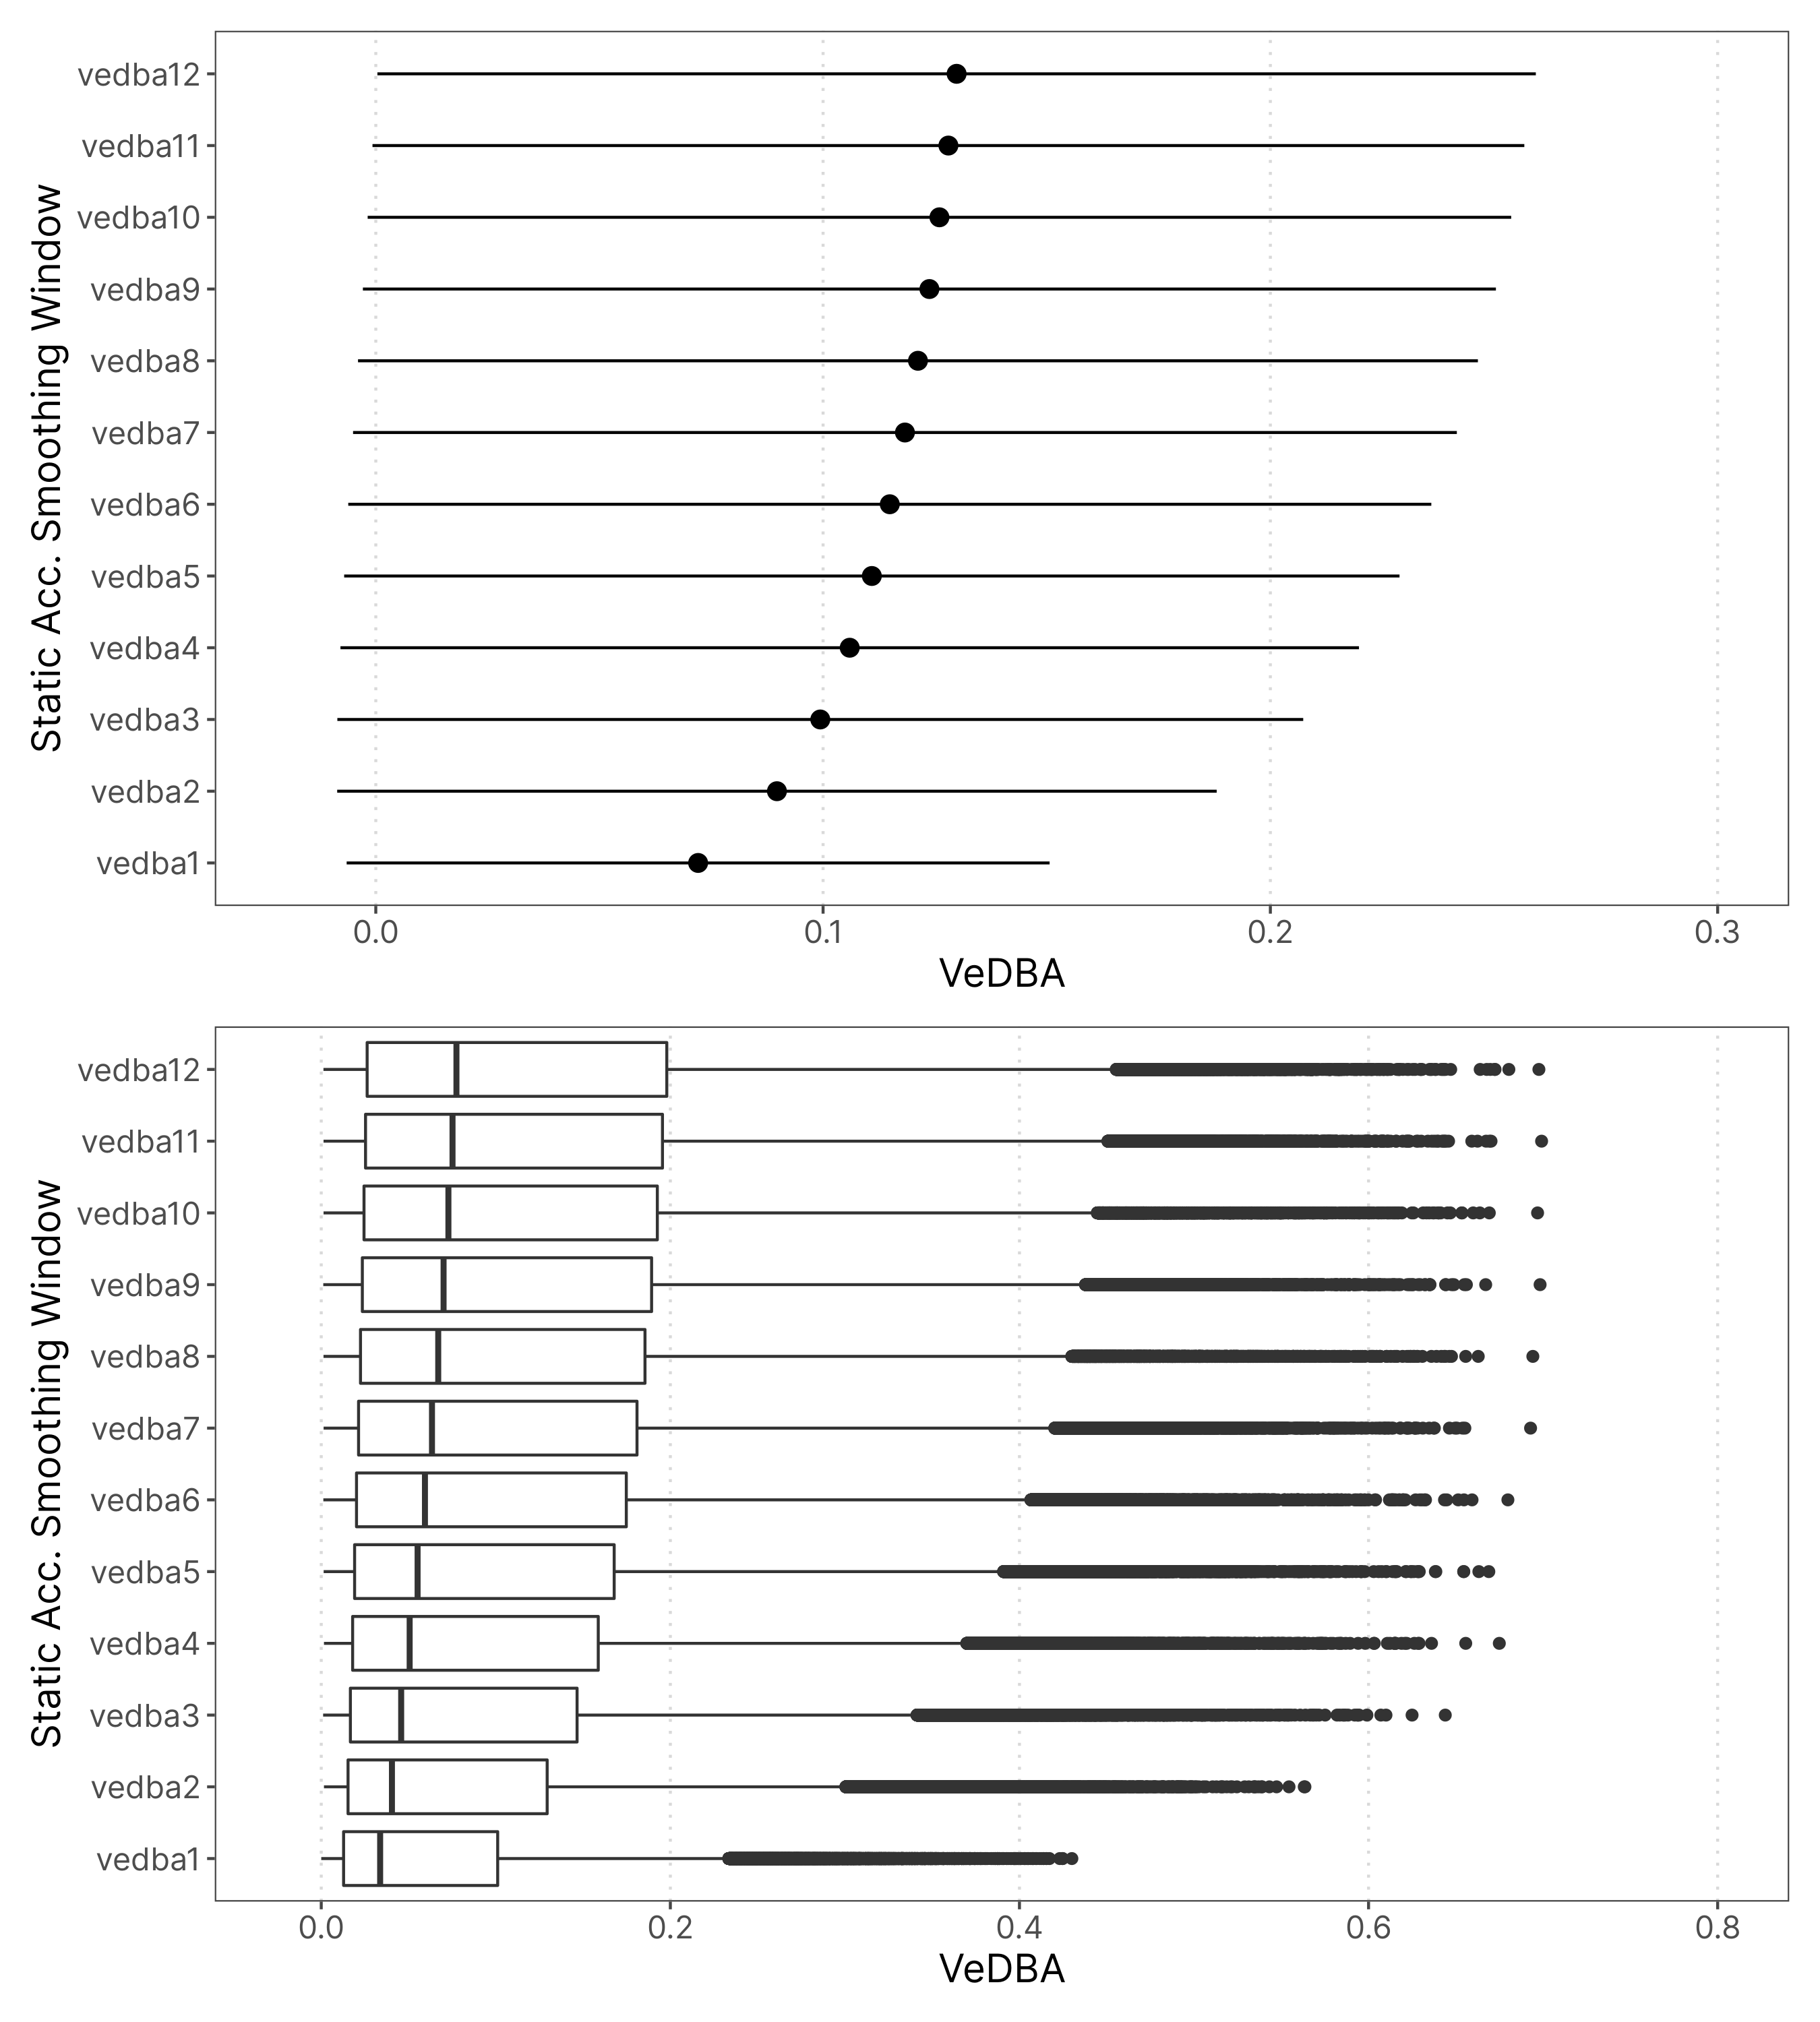
\includegraphics[width=1\linewidth]{../04_figures/appendix/plot_smoothing_window} \end{center}

  \hypertarget{exploratory-vedba-data-analysis}{%
  \chapter{Exploratory VeDBA data Analysis}\label{exploratory-vedba-data-analysis}}

  \hypertarget{hmm-aic}{%
  \chapter{HMM AIC}\label{hmm-aic}}
  \begin{itemize}
  \tightlist
  \item
    Adicionar o LL
  \end{itemize}
  \begin{table}[!h]
  \centering
  \begin{tabular}{ccc}
  \toprule
  Model & Formula & AIC\\
  \midrule
  m2 & \textasciitilde{}season & -935612.2\\
  m1 & \textasciitilde{}1 & -934800.8\\
  \bottomrule
  \end{tabular}
  \end{table}
  \hypertarget{hmm-estimated-parameters}{%
  \chapter{HMM Estimated Parameters}\label{hmm-estimated-parameters}}
  \begin{table}[!h]

  \caption{\label{tab:appendix-parameters}Gamma State-dependent distribution parameters, mean and standard deviation, estimated by a three-state Hidden Markov Model.}
  \centering
  \begin{tabular}[t]{cccc}
  \toprule
  Parameter & State & Estimate & CI\\
  \midrule
  mean & Rest & 0.018 & {}[0.018, 0.018]\\
  mean & Medium & 0.116 & {}[0.116, 0.117]\\
  mean & High & 0.327 & {}[0.326, 0.328]\\
  sd & Rest & 0.010 & {}[0.01, 0.01]\\
  sd & Medium & 0.051 & {}[0.05, 0.051]\\
  \addlinespace
  sd & High & 0.087 & {}[0.086, 0.087]\\
  \bottomrule
  \end{tabular}
  \end{table}
  \hypertarget{hmm-pseudo-residuals}{%
  \chapter{HMM Pseudo-residuals}\label{hmm-pseudo-residuals}}
  \begin{center}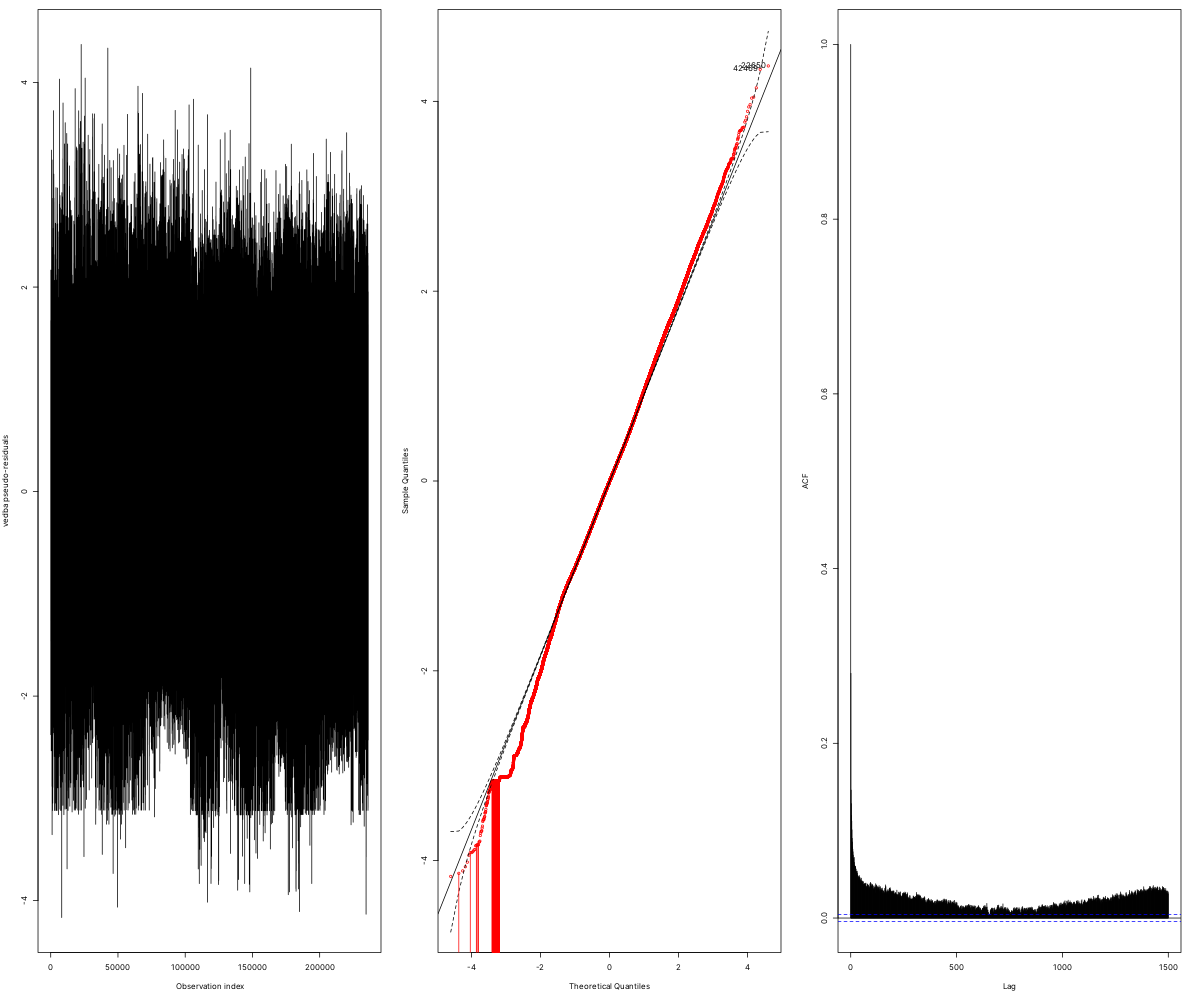
\includegraphics[width=1\linewidth]{../04_figures/residuals/m2_PR} \end{center}

  \hypertarget{individual-vedba-actograms}{%
  \chapter{Individual VeDBA Actograms}\label{individual-vedba-actograms}}
  \begin{center}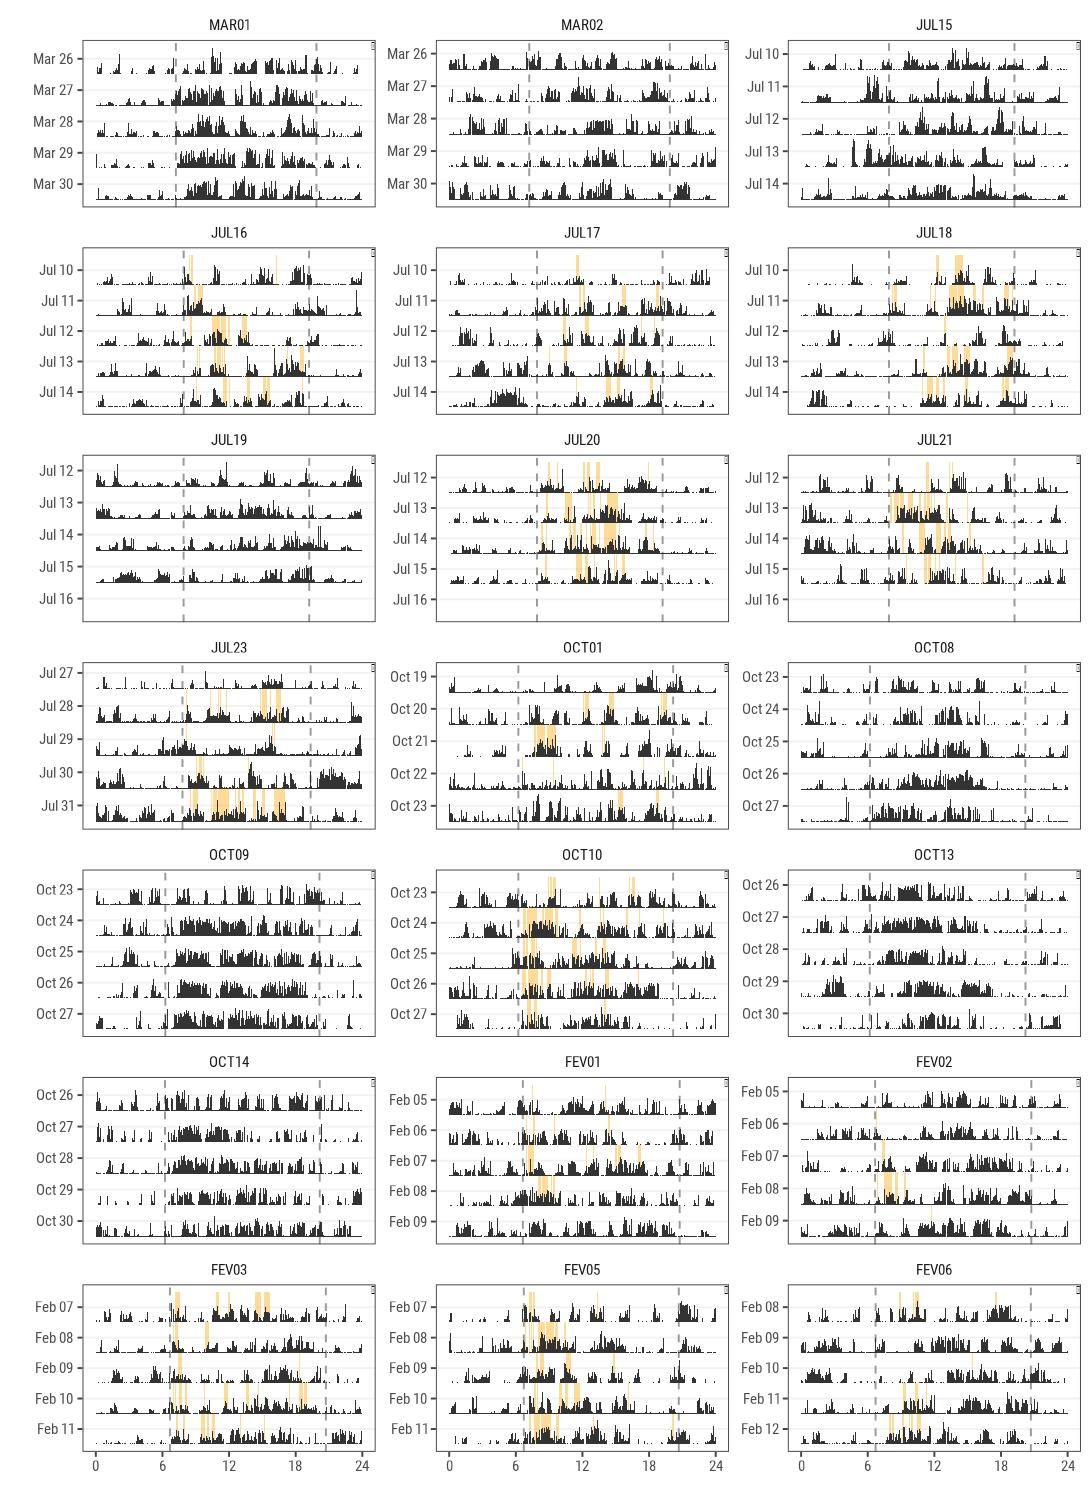
\includegraphics[width=0.95\linewidth]{../04_figures/actograms/actograms_vedba} \end{center}

  \hypertarget{individual-high-activity-actograms}{%
  \chapter{Individual High Activity Actograms}\label{individual-high-activity-actograms}}
  \begin{center}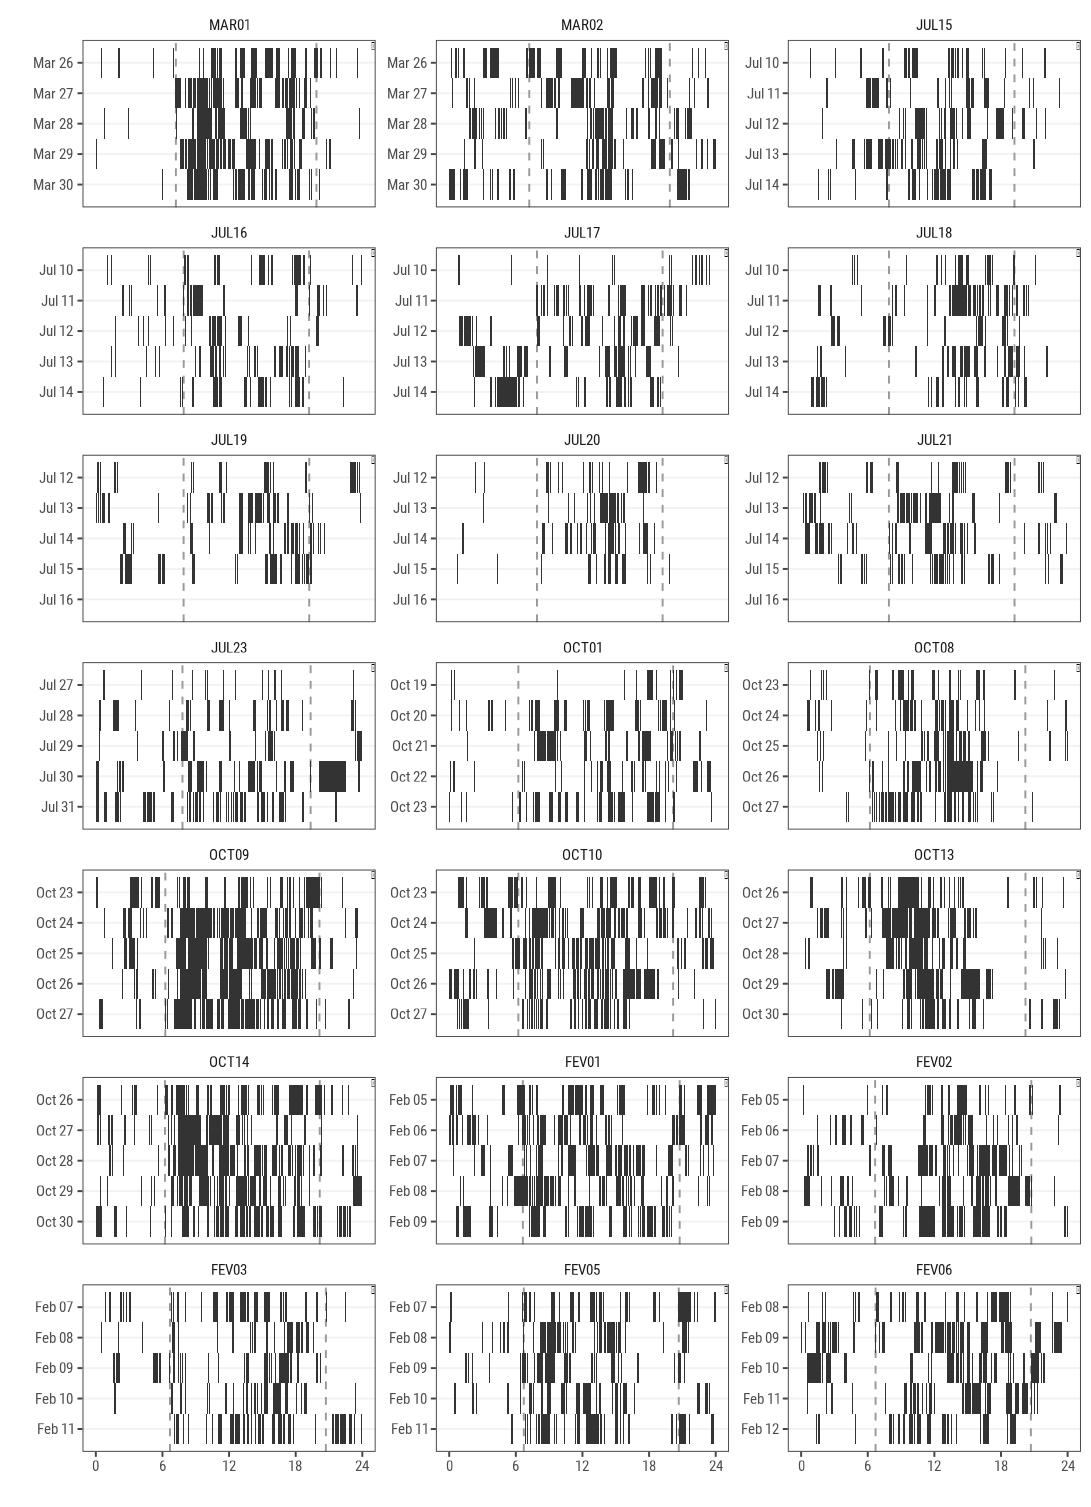
\includegraphics[width=0.95\linewidth]{../04_figures/actograms/actograms_high} \end{center}

  \hypertarget{individual-medium-activity-actograms}{%
  \chapter{Individual Medium Activity Actograms}\label{individual-medium-activity-actograms}}
  \begin{center}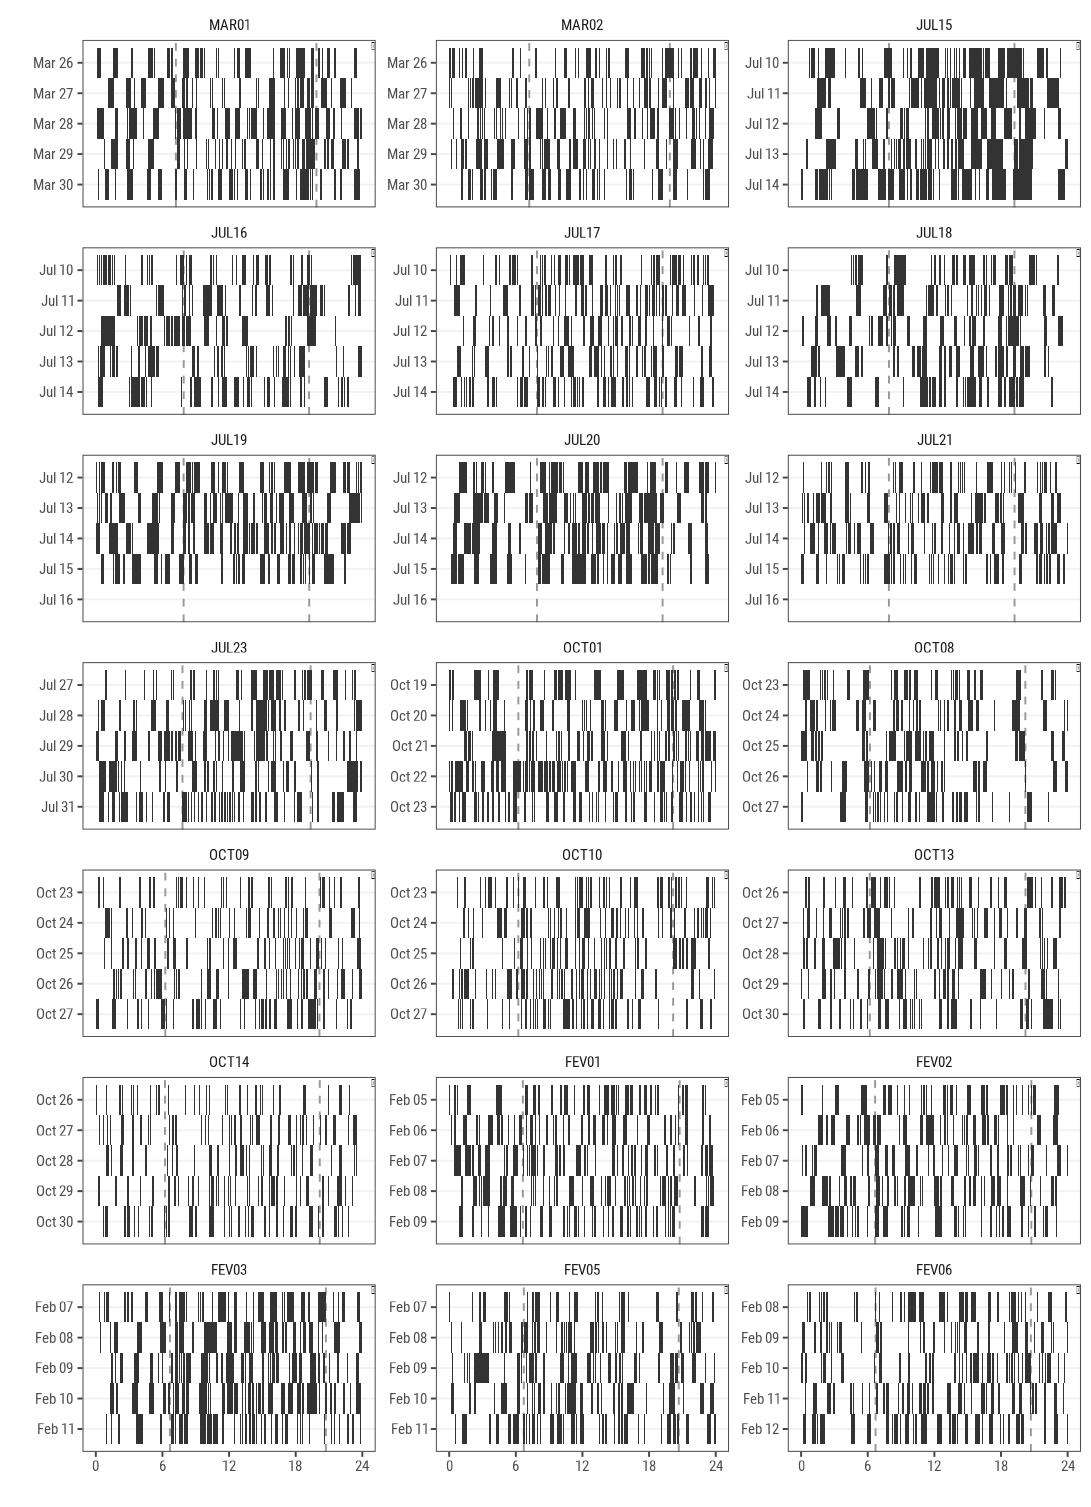
\includegraphics[width=0.95\linewidth]{../04_figures/actograms/actograms_medium} \end{center}

  \hypertarget{individual-rhythmicity-plots}{%
  \chapter{Individual Rhythmicity Plots}\label{individual-rhythmicity-plots}}
  \begin{center}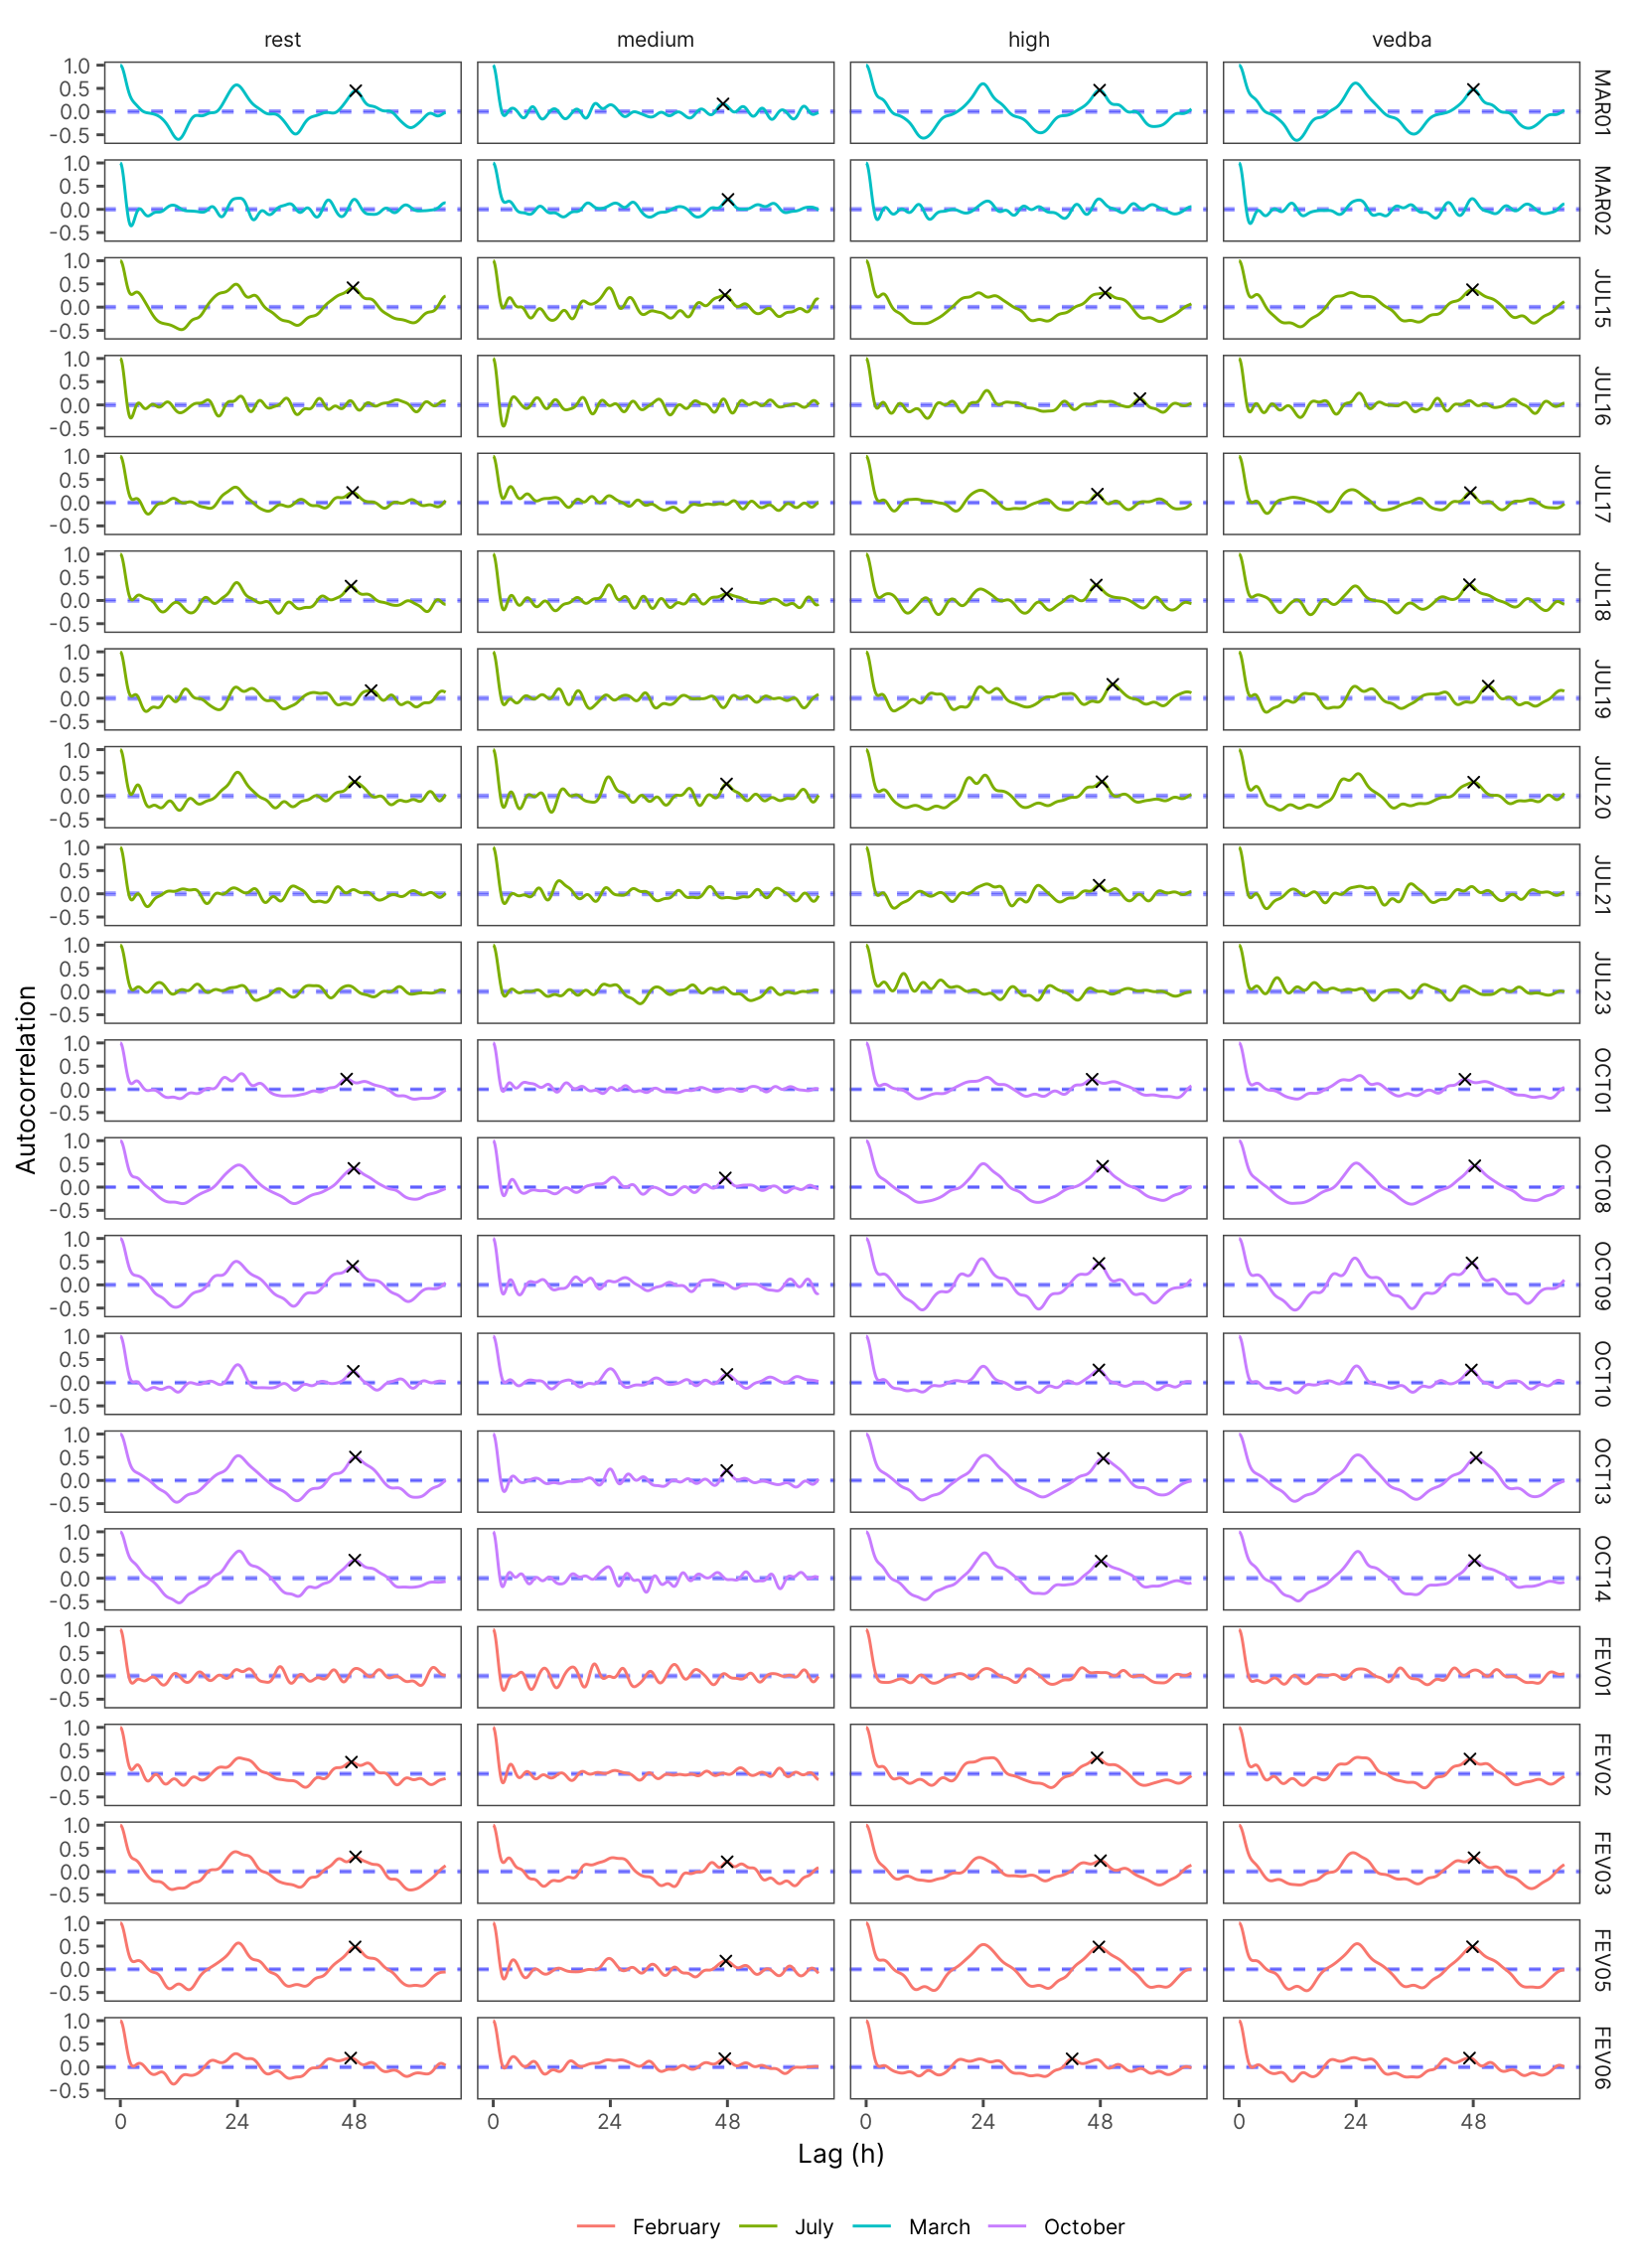
\includegraphics[width=22.96in]{../04_figures/ACF/acf_plot} \end{center}

  \hypertarget{individual-period-estimation}{%
  \chapter{Individual Period Estimation}\label{individual-period-estimation}}
  \begin{center}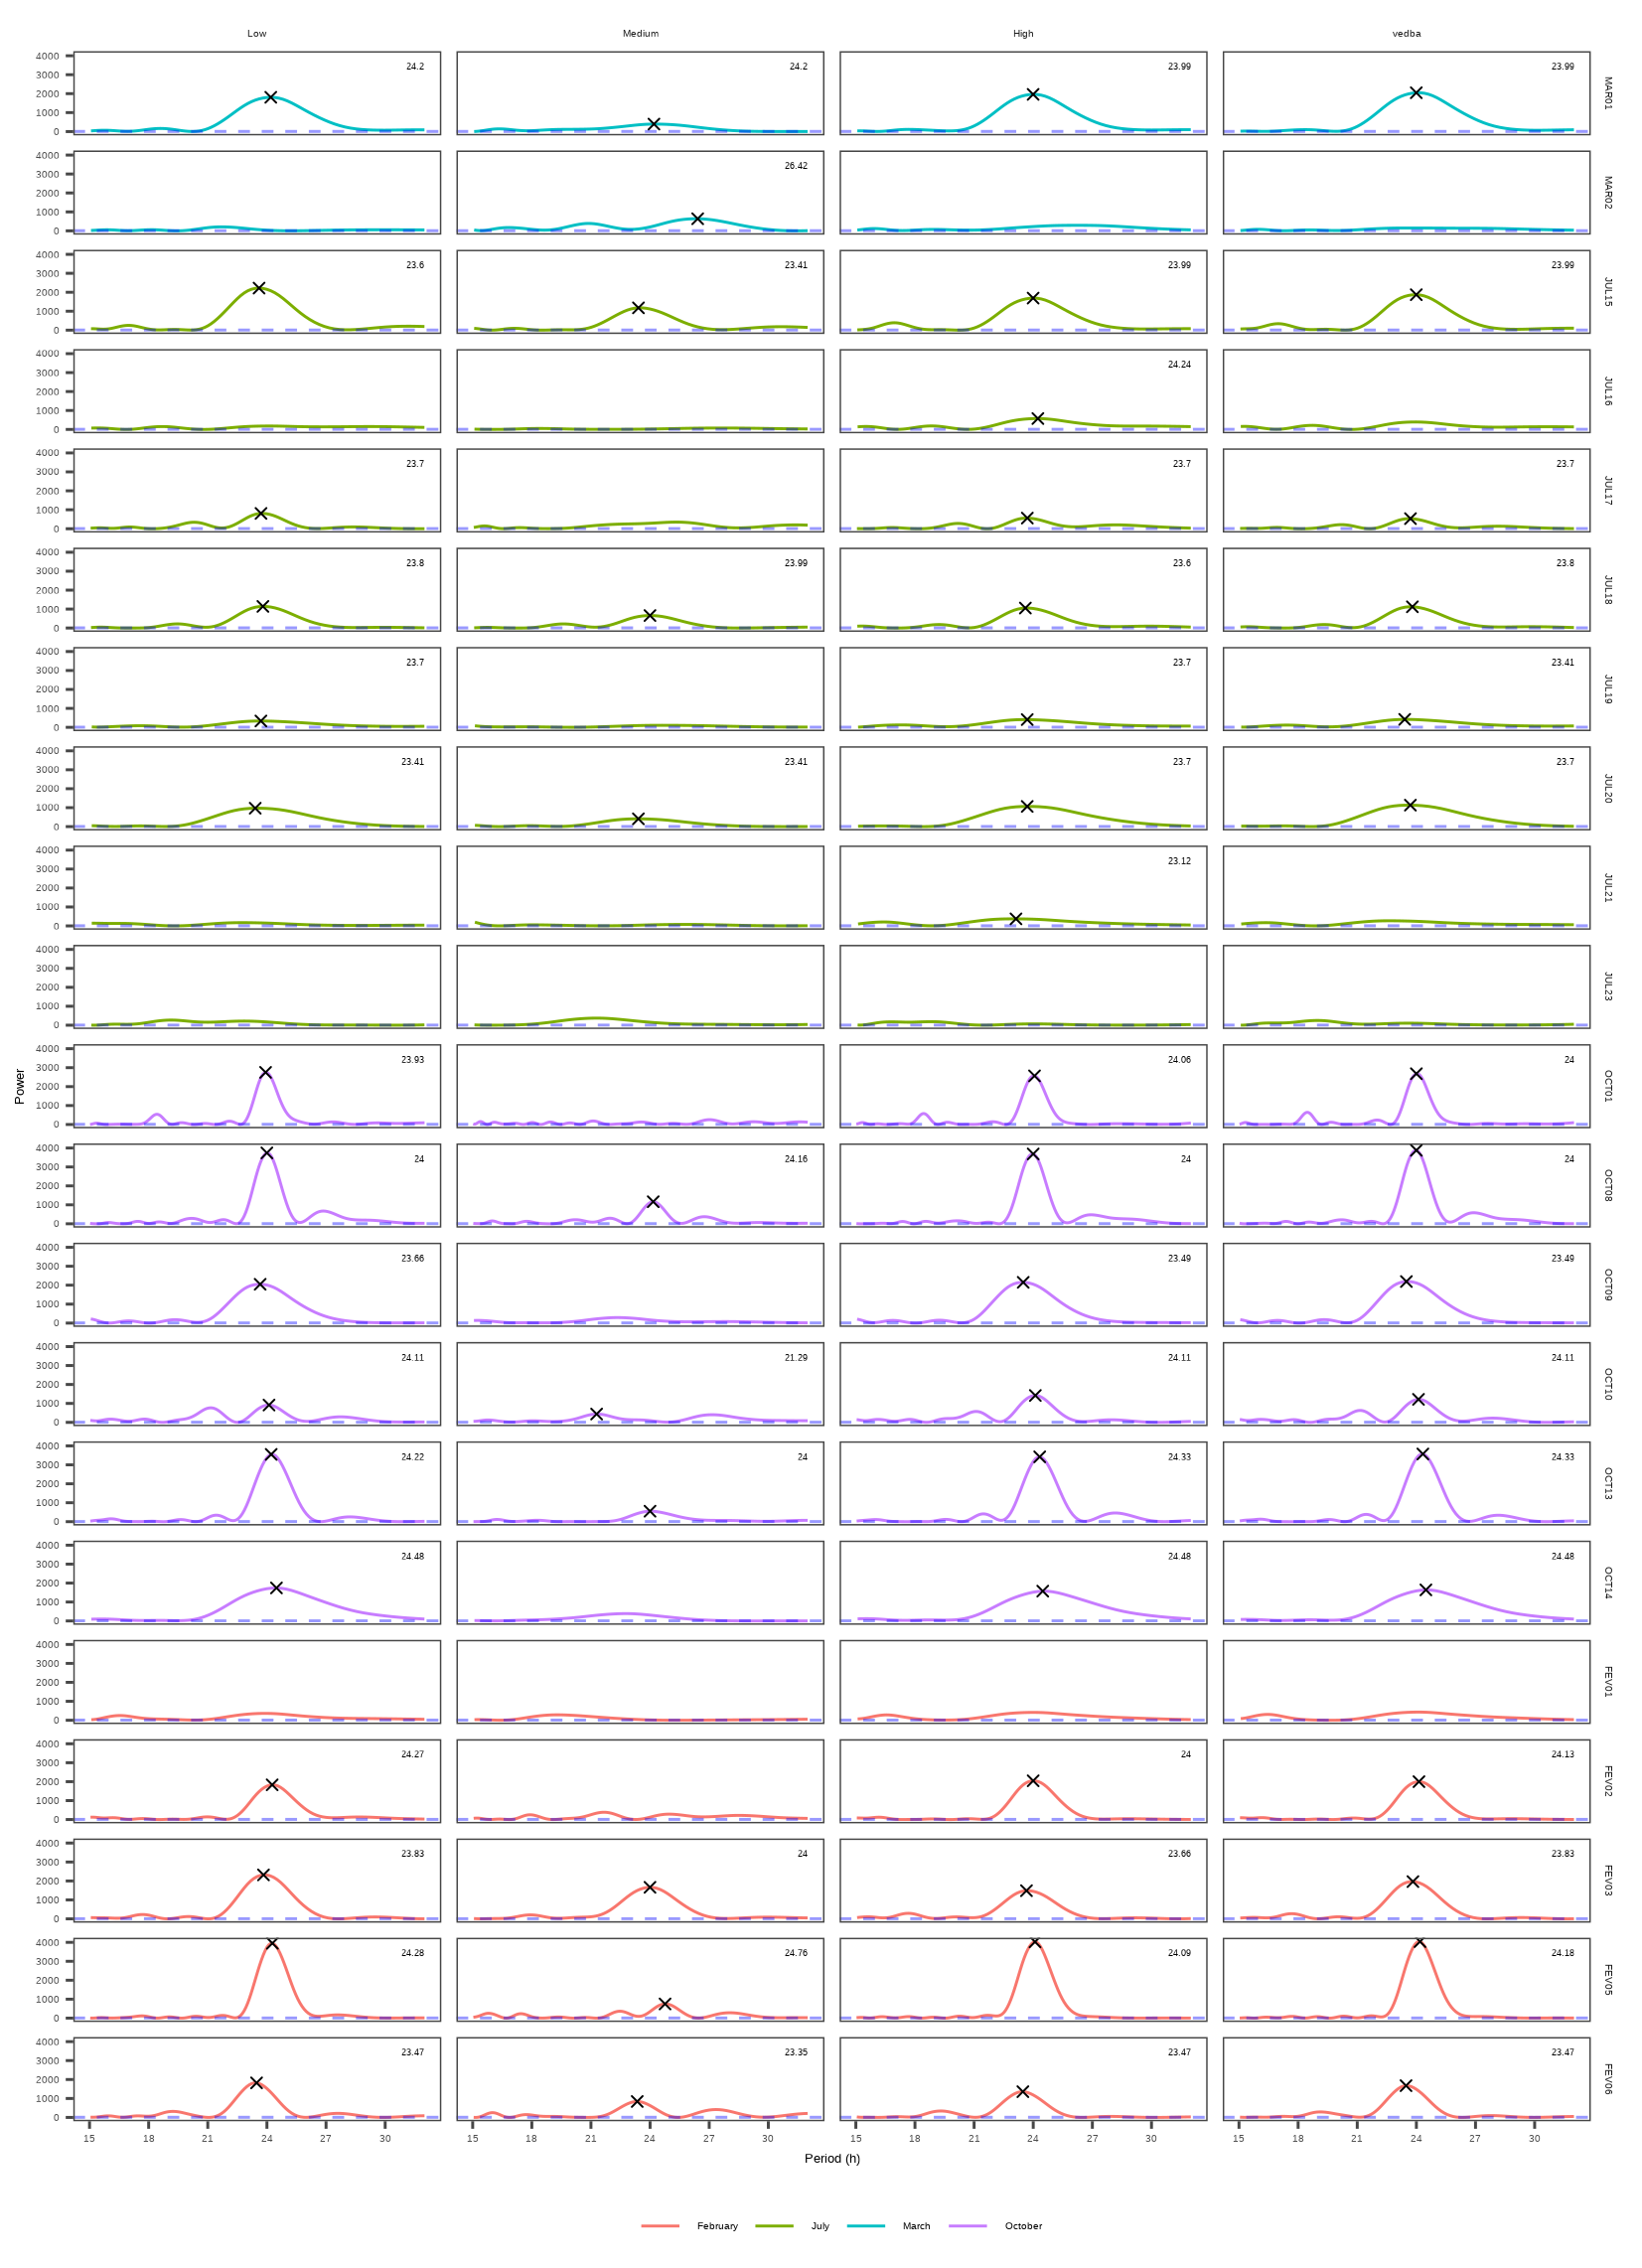
\includegraphics[width=22.96in]{../04_figures/periodogram/periodogram} \end{center}

  \backmatter
  \bibliographystyle{$biblio-style$}
  \bibliography{thesis}

  \hypertarget{references}{%
  \chapter*{References}\label{references}}
  \addcontentsline{toc}{chapter}{References}

  \noindent

  \setlength{\parindent}{-0.20in}
  \setlength{\leftskip}{0.20in}
  \setlength{\parskip}{8pt}

  \hypertarget{refs}{}
  \begin{CSLReferences}{1}{0}
  \leavevmode\vadjust pre{\hypertarget{ref-abraham2009}{}}%
  Abraham, E., H.F. del Valle, F. Roig, L. Torres, J.O. Ares, F. Coronato, and R. Godagnone. 2009. {``Overview of the Geography of the Monte Desert Biome (Argentina).''} \emph{Journal of Arid Environments} 73 (2): 144--53. \url{https://doi.org/10.1016/j.jaridenv.2008.09.028}.

  \leavevmode\vadjust pre{\hypertarget{ref-amaya2016}{}}%
  Amaya, Juan Pablo, Juan I. Areta, Veronica S. Valentinuzzi, and Emmanuel Zufiaurre. 2016. {``Form and Function of Long-Range Vocalizations in a Neotropical Fossorial Rodent: The Anillaco Tuco-Tuco ( {\emph{Ctenomys}} Sp.).''} \emph{PeerJ} 4 (October): e2559. \url{https://doi.org/10.7717/peerj.2559}.

  \leavevmode\vadjust pre{\hypertarget{ref-aranda-rickert2014}{}}%
  Aranda-Rickert, Adriana, Patricia Diez, and Brigitte Marazzi. 2014. {``Extrafloral Nectar Fuels Ant Life in Deserts.''} \emph{AoB PLANTS} 6 (January). \url{https://doi.org/10.1093/aobpla/plu068}.

  \leavevmode\vadjust pre{\hypertarget{ref-aranda-rickert2011a}{}}%
  Aranda-Rickert, Adriana, and Sebastián Fracchia. 2011. {``Pogonomyrmexcunicularius as the Keystone Disperser of Elaiosome-Bearing Jatropha Excisa Seeds in Semi-Arid Argentina: Pogonomyrmex Cunicularius Ants as Keystone Seed Dispersers.''} \emph{Entomologia Experimentalis Et Applicata} 139 (2): 91--102. \url{https://doi.org/10.1111/j.1570-7458.2011.01111.x}.

  \leavevmode\vadjust pre{\hypertarget{ref-bivand2020}{}}%
  Bivand, Roger, and Nicholas Lewin-Koh. 2020. {``Maptools: Tools for Handling Spatial Objects.''} \url{https://CRAN.R-project.org/package=maptools}.

  \leavevmode\vadjust pre{\hypertarget{ref-bunn2008}{}}%
  Bunn, Andrew G. 2008. {``A Dendrochronology Program Library in R (dplR).''} \emph{Dendrochronologia} 26 (2): 115--24. \url{https://doi.org/10.1016/j.dendro.2008.01.002}.

  \leavevmode\vadjust pre{\hypertarget{ref-burnham2002}{}}%
  Burnham, Kenneth P., David Raymond Anderson, and Kenneth P. Burnham. 2002. \emph{Model Selection and Multimodel Inference: A Practical Information-Theoretic Approach}. 2nd ed. New York: Springer.

  \leavevmode\vadjust pre{\hypertarget{ref-dowse2009}{}}%
  Dowse, Harold B. 2009. {``Chapter 6 Analyses for Physiological and Behavioral Rhythmicity.''} In, 454:141--74. Elsevier. \url{https://doi.org/10.1016/S0076-6879(08)03806-8}.

  \leavevmode\vadjust pre{\hypertarget{ref-fracchia2011}{}}%
  Fracchia, S., L. Krapovickas, A. Aranda-Rickert, and V.S. Valentinuzzi. 2011. {``Dispersal of Arbuscular Mycorrhizal Fungi and Dark Septate Endophytes by Ctenomys Cf. Knighti (Rodentia) in the Northern Monte Desert of Argentina.''} \emph{Journal of Arid Environments} 75 (11): 1016--23. \url{https://doi.org/10.1016/j.jaridenv.2011.04.034}.

  \leavevmode\vadjust pre{\hypertarget{ref-activity2000}{}}%
  Halle, S., and Nils Chr Stenseth, eds. 2000. \emph{Activity Patterns in Small Mammals: An Ecological Approach}. Ecological Studies, v. 141. Berlin ; New York: Springer.

  \leavevmode\vadjust pre{\hypertarget{ref-hansw.borchers2019}{}}%
  Hans W. Borchers. 2019. {``Pracma: Practical Numerical Math Functions.''} \url{https://CRAN.R-project.org/package=pracma}.

  \leavevmode\vadjust pre{\hypertarget{ref-jannetti2019}{}}%
  Jannetti, Milene G., C. Loren Buck, Veronica S. Valentinuzzi, and Gisele A. Oda. 2019. {``Day and Night in the Subterranean: Measuring Daily Activity Patterns of Subterranean Rodents (Ctenomys Aff. Knighti) Using Bio-Logging.''} \emph{Conservation Physiology} 7 (1). \url{https://doi.org/10.1093/conphys/coz044}.

  \leavevmode\vadjust pre{\hypertarget{ref-langrock2012}{}}%
  Langrock, Roland, Ruth King, Jason Matthiopoulos, Len Thomas, Daniel Fortin, and Juan M. Morales. 2012. {``Flexible and Practical Modeling of Animal Telemetry Data: Hidden Markov Models and Extensions.''} \emph{Ecology} 93 (11): 2336--42. \url{https://doi.org/10.1890/11-2241.1}.

  \leavevmode\vadjust pre{\hypertarget{ref-leise2017}{}}%
  Leise, Tanya L. 2017. {``Analysis of Nonstationary Time Series for Biological Rhythms Research.''} \emph{Journal of Biological Rhythms} 32 (3): 187--94. \url{https://doi.org/10.1177/0748730417709105}.

  \leavevmode\vadjust pre{\hypertarget{ref-leosbarajas2017}{}}%
  Leos-Barajas, Vianey, Theoni Photopoulou, Roland Langrock, Toby A. Patterson, Yuuki Y. Watanabe, Megan Murgatroyd, and Yannis P. Papastamatiou. 2017. {``Analysis of Animal Accelerometer Data Using Hidden Markov Models.''} Edited by Robert B. O'Hara. \emph{Methods in Ecology and Evolution} 8 (2): 161--73. \url{https://doi.org/10.1111/2041-210X.12657}.

  \leavevmode\vadjust pre{\hypertarget{ref-levine2002}{}}%
  Levine, Joel D, Pablo Funes, Harold B Dowse, and Jeffrey C Hall. 2002. {``Signal Analysis of Behavioral and Molecular Cycles.''} \emph{BMC Neuroscience}, 25.

  \leavevmode\vadjust pre{\hypertarget{ref-mcclintock2020}{}}%
  McClintock, Brett T., Roland Langrock, Olivier Gimenez, Emmanuelle Cam, David L. Borchers, Richard Glennie, and Toby A. Patterson. 2020. {``Uncovering Ecological State Dynamics with Hidden Markov Models.''} Edited by Tim Coulson. \emph{Ecology Letters} 23 (12): 1878--1903. \url{https://doi.org/10.1111/ele.13610}.

  \leavevmode\vadjust pre{\hypertarget{ref-mcclintock2021}{}}%
  McClintock, Brett T, and Theo Michelot. 2021. {``momentuHMM: R Package for Analysis of Telemetry Data Using Generalized Multivariate Hidden Markov Models of Animal Movement,''} 155.

  \leavevmode\vadjust pre{\hypertarget{ref-michelot2019}{}}%
  Michelot, Theo, and Roland Langrock. 2019. {``A Short Guide to Choosing Initial Parameter Values for the Estimation in moveHMM,''} 10.

  \leavevmode\vadjust pre{\hypertarget{ref-papastamatiou2018}{}}%
  Papastamatiou, Yannis P., Yuuki Y. Watanabe, Urška Demšar, Vianey Leos-Barajas, Darcy Bradley, Roland Langrock, Kevin Weng, Christopher G. Lowe, Alan M. Friedlander, and Jennifer E. Caselle. 2018. {``Activity Seascapes Highlight Central Place Foraging Strategies in Marine Predators That Never Stop Swimming.''} \emph{Movement Ecology} 6 (1): 9. \url{https://doi.org/10.1186/s40462-018-0127-3}.

  \leavevmode\vadjust pre{\hypertarget{ref-patterson2019}{}}%
  Patterson, Allison, Hugh Grant Gilchrist, Lorraine Chivers, Scott Hatch, and Kyle Elliott. 2019. {``A Comparison of Techniques for Classifying Behavior from Accelerometers for Two Species of Seabird.''} \emph{Ecology and Evolution} 9 (6): 3030--45. \url{https://doi.org/10.1002/ece3.4740}.

  \leavevmode\vadjust pre{\hypertarget{ref-patterson2009}{}}%
  Patterson, Toby A., Marinelle Basson, Mark V. Bravington, and John S. Gunn. 2009. {``Classifying Movement Behaviour in Relation to Environmental Conditions Using Hidden Markov Models.''} \emph{Journal of Animal Ecology} 78 (6): 1113--23. \url{https://doi.org/10.1111/j.1365-2656.2009.01583.x}.

  \leavevmode\vadjust pre{\hypertarget{ref-pohle2017}{}}%
  Pohle, Jennifer, Roland Langrock, Floris M. van Beest, and Niels Martin Schmidt. 2017. {``Selecting the Number of States in Hidden Markov Models: Pragmatic Solutions Illustrated Using Animal Movement.''} \emph{Journal of Agricultural, Biological and Environmental Statistics} 22 (3): 270--93. \url{https://doi.org/10.1007/s13253-017-0283-8}.

  \leavevmode\vadjust pre{\hypertarget{ref-qasem2012}{}}%
  Qasem, Lama, Antonia Cardew, Alexis Wilson, Iwan Griffiths, Lewis G. Halsey, Emily L. C. Shepard, Adrian C. Gleiss, and Rory Wilson. 2012. {``Tri-Axial Dynamic Acceleration as a Proxy for Animal Energy Expenditure; Should We Be Summing Values or Calculating the Vector?''} \emph{PLOS ONE} 7 (2): e31187. \url{https://doi.org/10.1371/journal.pone.0031187}.

  \leavevmode\vadjust pre{\hypertarget{ref-rcoreteam2020}{}}%
  R Core Team. 2020. {``R: A Language and Environment for Statistical Computing.''} \url{https://www.R-project.org/.}

  \leavevmode\vadjust pre{\hypertarget{ref-ruf1999}{}}%
  Ruf, T. 1999. {``The Lomb-Scargle Periodogram in Biological Rhythm Research: Analysis of Incomplete and Unequally Spaced Time-Series.''} \emph{Biological Rhythm Research} 30 (2): 178--201. \url{https://doi.org/10.1076/brhm.30.2.178.1422}.

  \leavevmode\vadjust pre{\hypertarget{ref-shepard2008}{}}%
  Shepard, Elc, Rp Wilson, Lg Halsey, F Quintana, A Gómez Laich, Ac Gleiss, N Liebsch, Ae Myers, and B Norman. 2008. {``Derivation of Body Motion via Appropriate Smoothing of Acceleration Data.''} \emph{Aquatic Biology} 4 (December): 235--41. \url{https://doi.org/10.3354/ab00104}.

  \leavevmode\vadjust pre{\hypertarget{ref-tomotani2012}{}}%
  Tomotani, Barbara M., Danilo E. F. L. Flores, Patrícia Tachinardi, José D. Paliza, Gisele A. Oda, and Verônica S. Valentinuzzi. 2012. {``Field and Laboratory Studies Provide Insights into the Meaning of Day-Time Activity in a Subterranean Rodent (Ctenomys Aff. Knighti), the Tuco-Tuco.''} Edited by Ralph E. Mistlberger. \emph{PLoS ONE} 7 (5): e37918. \url{https://doi.org/10.1371/journal.pone.0037918}.

  \leavevmode\vadjust pre{\hypertarget{ref-valentinuzzi2009}{}}%
  Valentinuzzi, Verónica Sandra, Gisele Akemi Oda, John Fontenele Araújo, and Martin Roland Ralph. 2009. {``Circadian Pattern of Wheel{-}Running Activity of a South American Subterranean Rodent ( {\emph{Ctenomys Cf Knightii}} ).''} \emph{Chronobiology International} 26 (1): 14--27. \url{https://doi.org/10.1080/07420520802686331}.

  \leavevmode\vadjust pre{\hypertarget{ref-vandekerk2015}{}}%
  van de Kerk, Madelon, David P. Onorato, Marc A. Criffield, Benjamin M. Bolker, Ben C. Augustine, Scott A. McKinley, and Madan K. Oli. 2015. {``Hidden Semi-Markov Models Reveal Multiphasic Movement of the Endangered Florida Panther.''} Edited by Tim Coulson. \emph{Journal of Animal Ecology} 84 (2): 576--85. \url{https://doi.org/10.1111/1365-2656.12290}.

  \leavevmode\vadjust pre{\hypertarget{ref-williams2014}{}}%
  Williams, Cory T., Kathryn Wilsterman, Amanda D. Kelley, André R. Breton, Herbert Stark, Murray M. Humphries, Andrew G. McAdam, Brian M. Barnes, Stan Boutin, and C. Loren Buck. 2014. {``Light Loggers Reveal Weather-Driven Changes in the Daily Activity Patterns of Arboreal and Semifossorial Rodents.''} \emph{Journal of Mammalogy} 95 (6): 1230--39. \url{https://doi.org/10.1644/14-MAMM-A-062}.

  \leavevmode\vadjust pre{\hypertarget{ref-williams2016}{}}%
  Williams, Cory T., Kathryn Wilsterman, Victor Zhang, Jeanette Moore, Brian M. Barnes, and C. Loren Buck. 2016. {``The Secret Life of Ground Squirrels: Accelerometry Reveals Sex-Dependent Plasticity in Above-Ground Activity.''} \emph{Royal Society Open Science} 3 (9): 160404. \url{https://doi.org/10.1098/rsos.160404}.

  \leavevmode\vadjust pre{\hypertarget{ref-wilson2008}{}}%
  Wilson, Rory P., Craig R. White, Flavio Quintana, Lewis G. Halsey, Nikolai Liebsch, Graham R. Martin, and Patrick J. Butler. 2008. {``Moving Towards Acceleration for Estimates of Activity-Specific Metabolic Rate in Free-Living Animals: The Case of the Cormorant.''} \emph{Journal of Animal Ecology}, November, 1081--90. \url{https://doi.org/10.1111/j.1365-2656.2006.01127.x@10.1111/(ISSN)1365-2656.BIOTEL}.

  \leavevmode\vadjust pre{\hypertarget{ref-zucchini2016}{}}%
  Zucchini, Walter, Iain MacDonald, and Roland Langrock. 2016. \emph{Hidden Markov Models for Time Series - An Introduction Using R}. Vol. 43.

  \end{CSLReferences}
\end{document}
